\documentclass{beamer}
\usepackage{ctex, hyperref}

% other packages
\usepackage{latexsym,amsmath,xcolor,multicol,booktabs,calligra}
\usepackage{graphicx,pstricks,listings,stackengine}
\usepackage{tsinghua}
\usepackage{subcaption}
\usepackage{tcolorbox}
\usepackage{siunitx}
\usepackage{physics}
\usepackage{bm}
\usepackage{lipsum}

\usefonttheme[onlymath]{serif}

\title{基于物理模拟的正颌手术术后外形预测}
\subtitle{毕业设计终期汇报}
\author{李钦 \\ 指导教师: 徐枫}
\institute{清华大学软件学院}
\date{2024 年 6 月 7 日}

\DeclareMathOperator{\dist}{dist}

\begin{document}

\kaishu

\begin{frame}
  \titlepage
\end{frame}

\begin{frame}
  \tableofcontents[sectionstyle=show,subsectionstyle=show/shaded/hide,subsubsectionstyle=show/shaded/hide]
\end{frame}

\section{研究问题}

\begin{frame}{研究问题}
  \begin{description}
    \item[应用场景] 正颌手术规划中, 预测术后患者的面部外形
    \item[输入] 术前患者的头部 CT 数据, 术后患者的颅骨模型
    \item[输出] 术后患者的面部模型
    \item[数据] 多组术前, 术后的患者 CT 数据
  \end{description}
\end{frame}

\section{三维模型重建}

\begin{frame}{三维模型重建}
  \begin{description}
    \item[目标] CT (voxel grid) $\to$ 四面体网格
    \item[步骤]
          \begin{enumerate}
            \item 构建模板网格模型
            \item 预处理 CT 数据
            \item 刚性配准
            \item 非刚性配准
            \item 使用 TetGen 进行四面体划分
          \end{enumerate}
  \end{description}
  \begin{figure}
    \centering
    \subcaptionbox{CT}{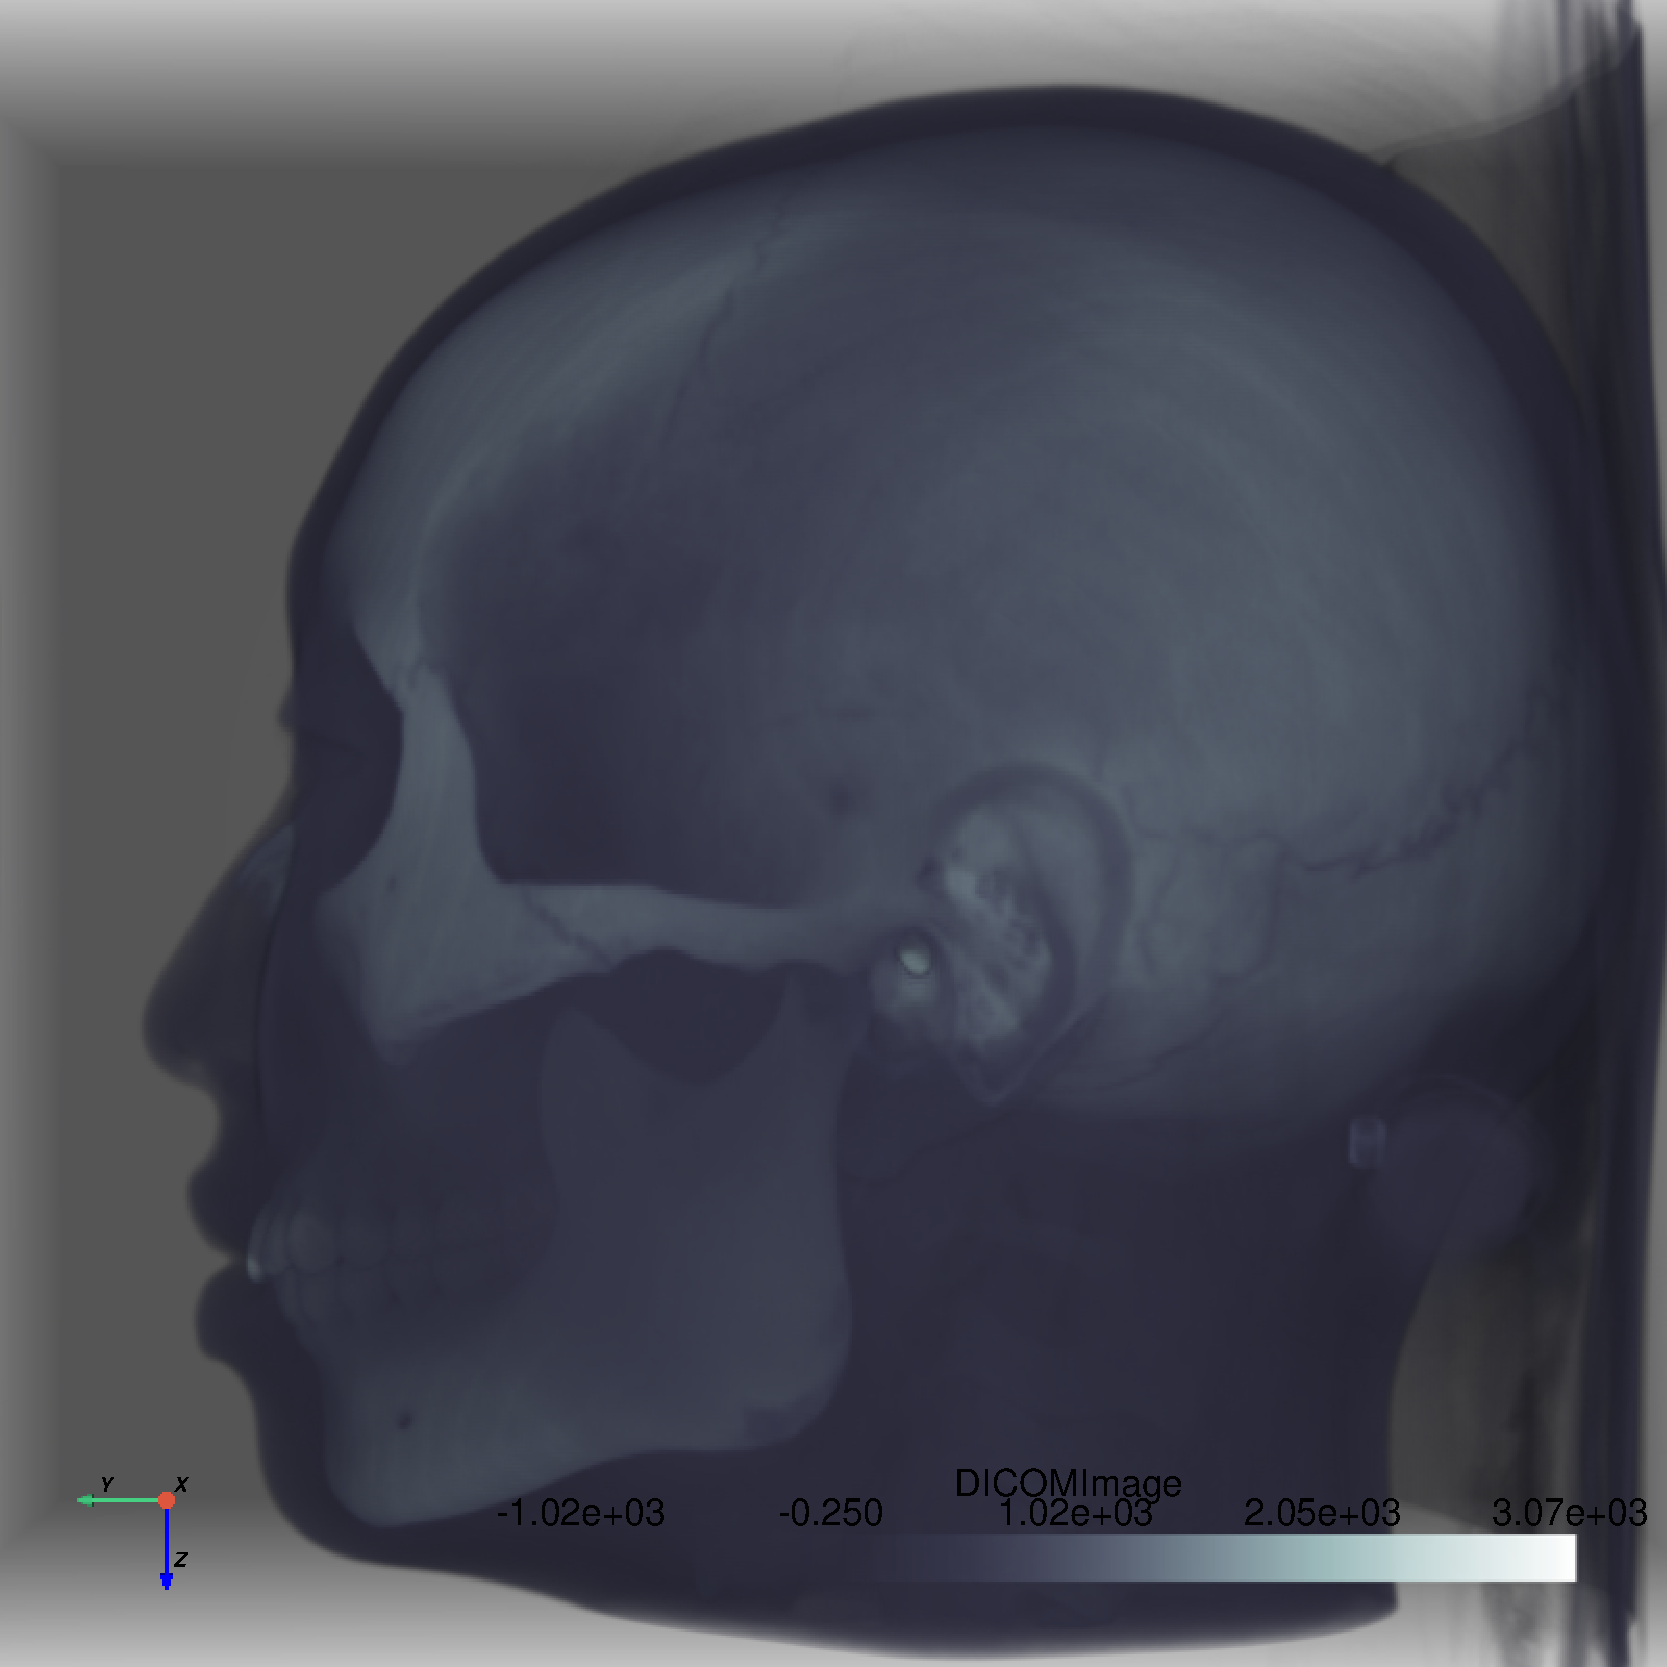
\includegraphics[height = 0.3 \linewidth]{fig/register/ct-lateral.pdf}} \quad
    \subcaptionbox{四面体网格}{\includegraphics[height = 0.3 \linewidth]{fig/tetra.png}}
  \end{figure}
\end{frame}

\begin{frame}{CT $\to$ 网格模型}
  \begin{enumerate}
    \item 对 CT 应用 Gaussian 平滑
    \item 提取等值曲面 (阈值: 软组织 \num{-200}, 骨骼 \num{200})
    \item 根据连接关系保留最大连通分量
  \end{enumerate}
  \begin{figure}
    \centering
    \subcaptionbox{CT}{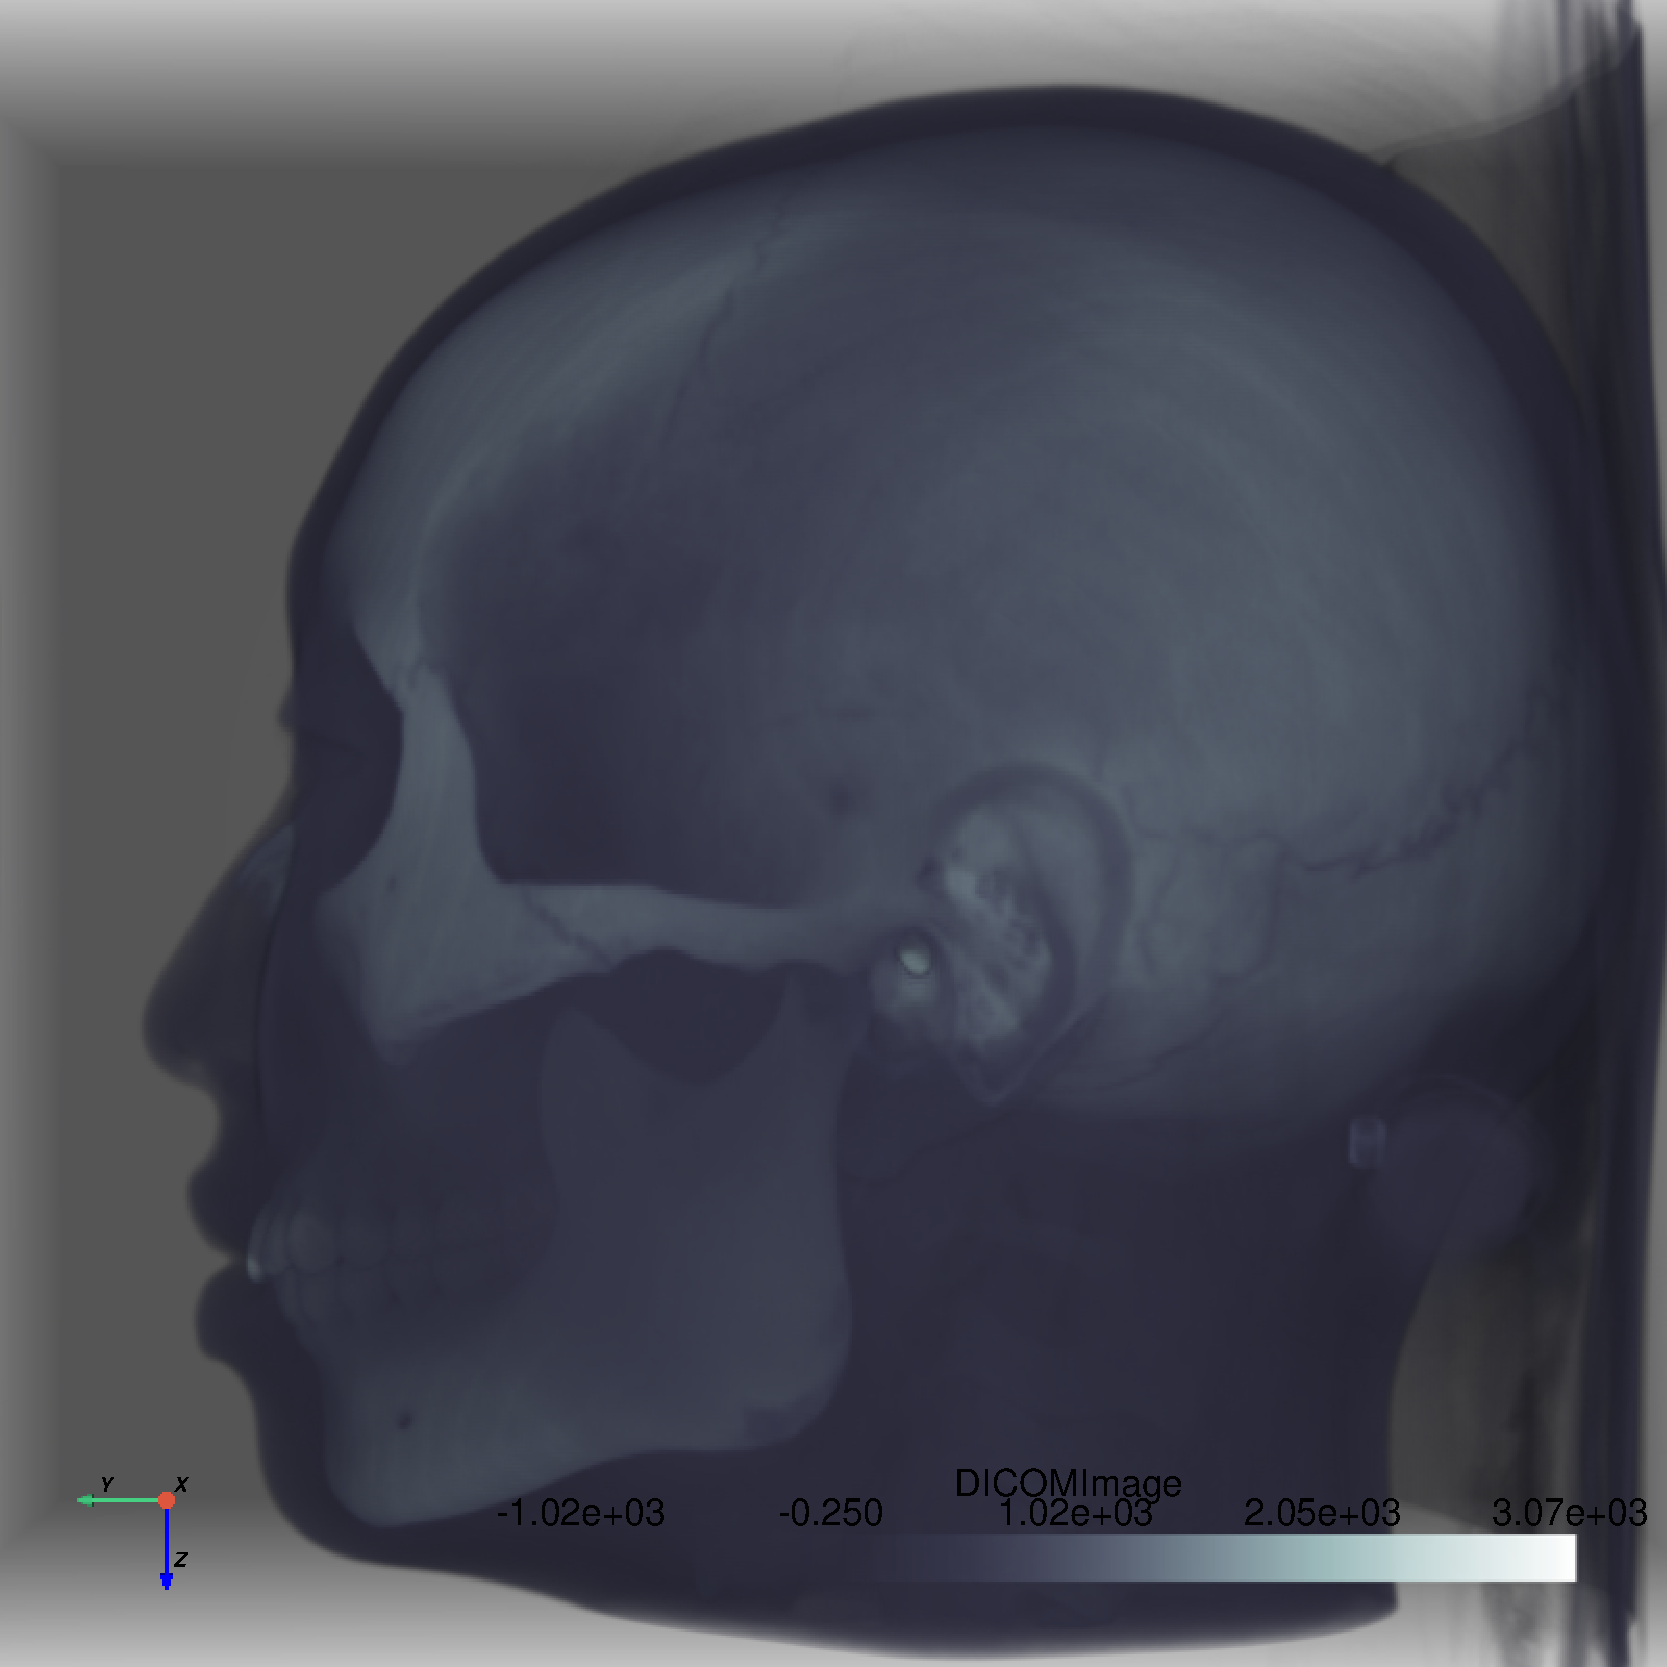
\includegraphics[height = 0.32 \linewidth]{fig/register/ct-lateral.pdf}}
    \subcaptionbox{面部}{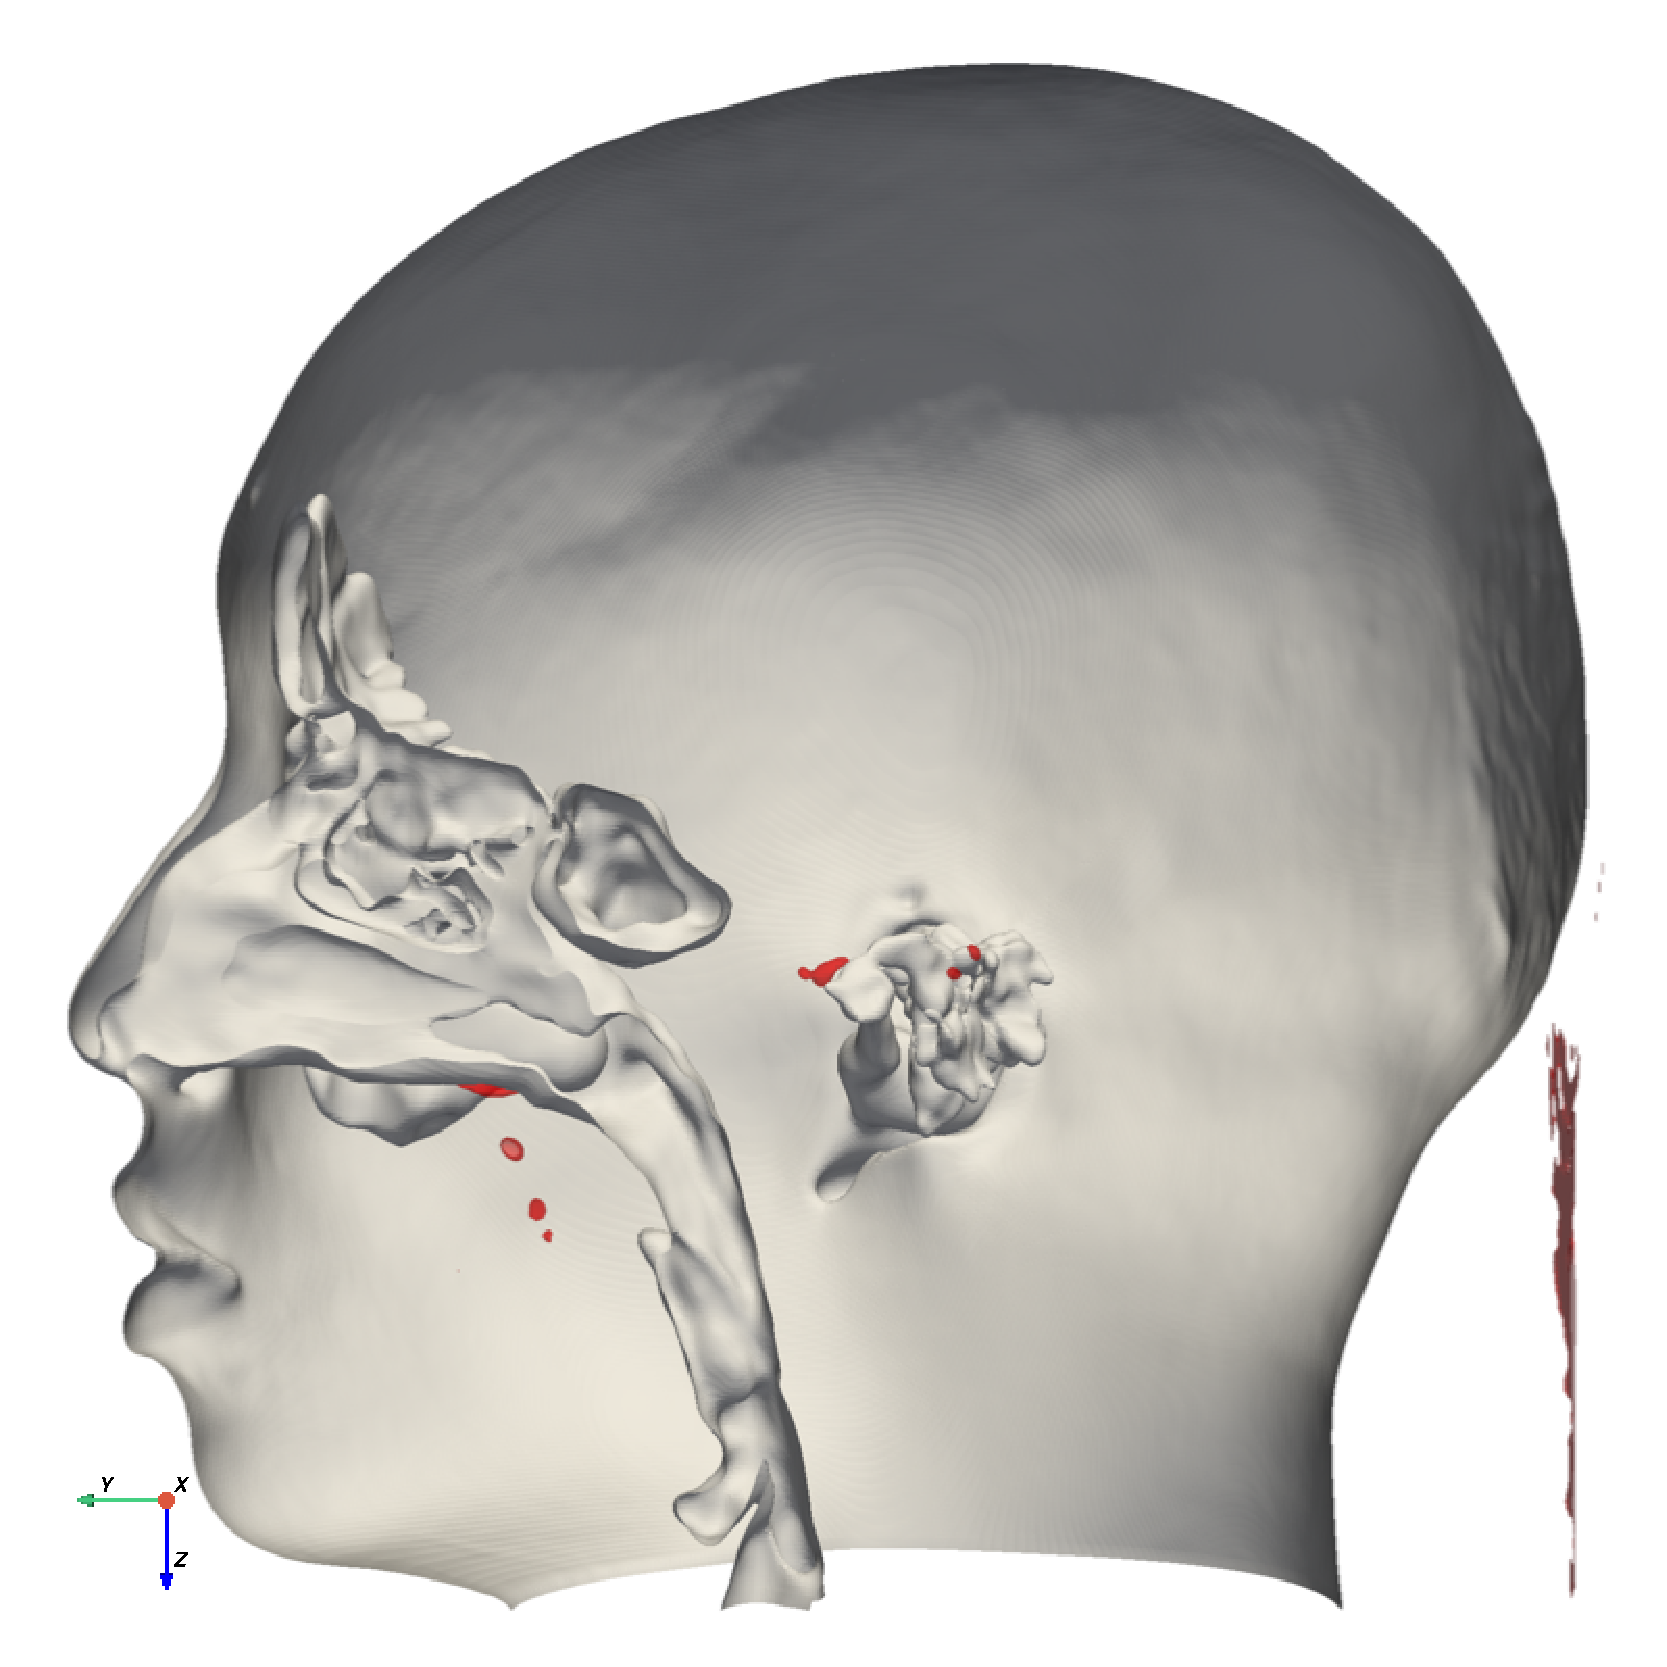
\includegraphics[height = 0.32 \linewidth]{fig/register/contour-face-gaussian-on.pdf}}
    \subcaptionbox{骨骼}{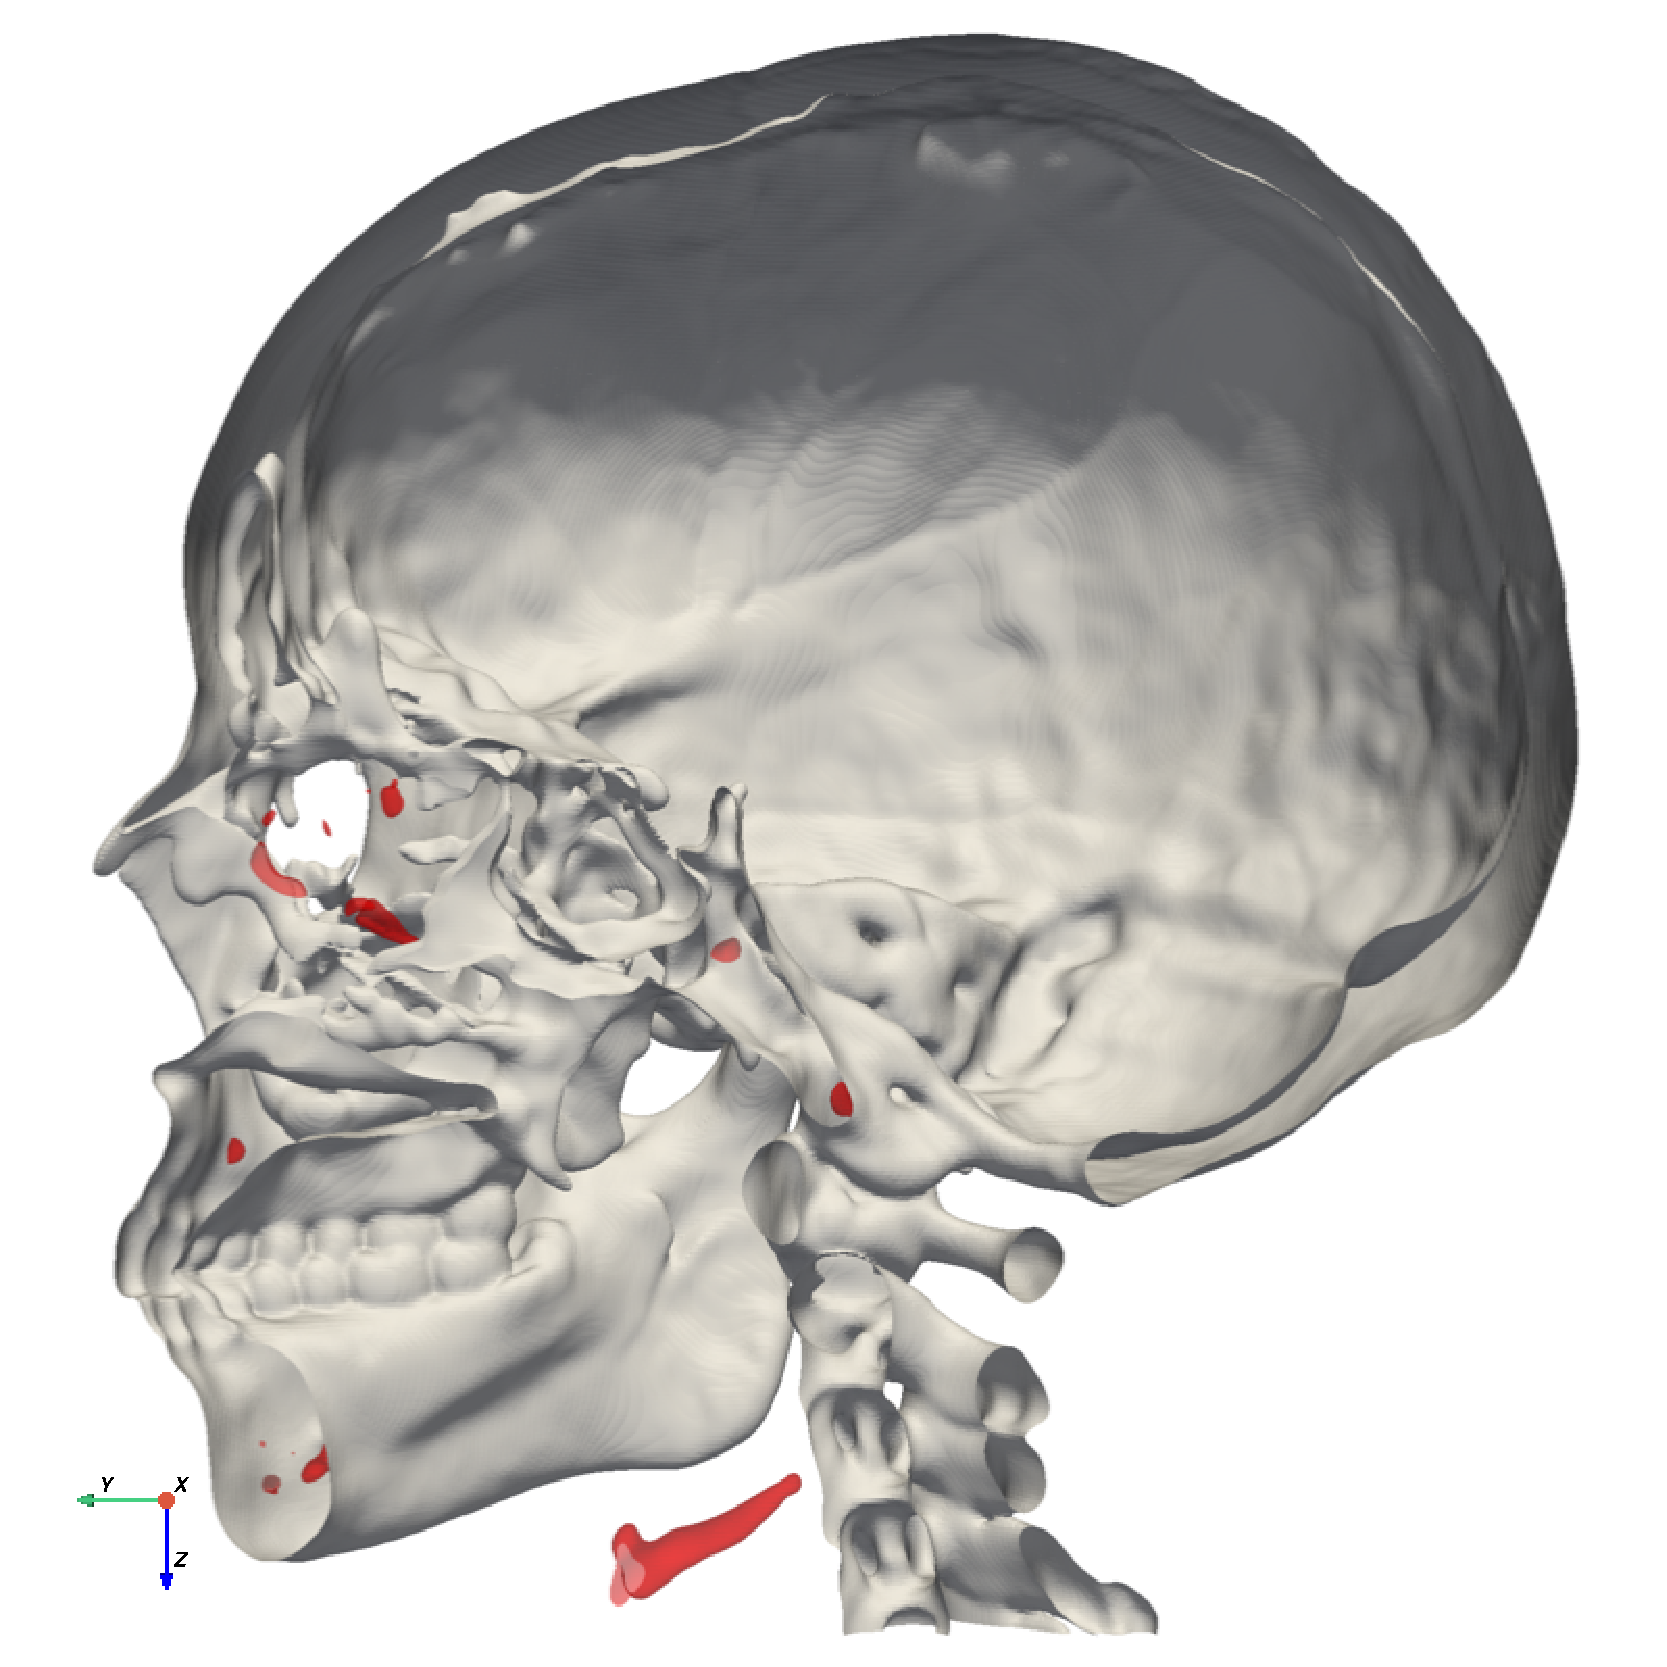
\includegraphics[height = 0.32 \linewidth]{fig/register/contour-skull-gaussian-on.pdf}}
  \end{figure}
\end{frame}

\begin{frame}{刚性配准}
  \begin{enumerate}
    \item 根据特征点估计初始的全局刚性变换
    \item 使用迭代最近邻 (ICP) 优化全局变换
  \end{enumerate}
  \begin{figure}
    \centering
    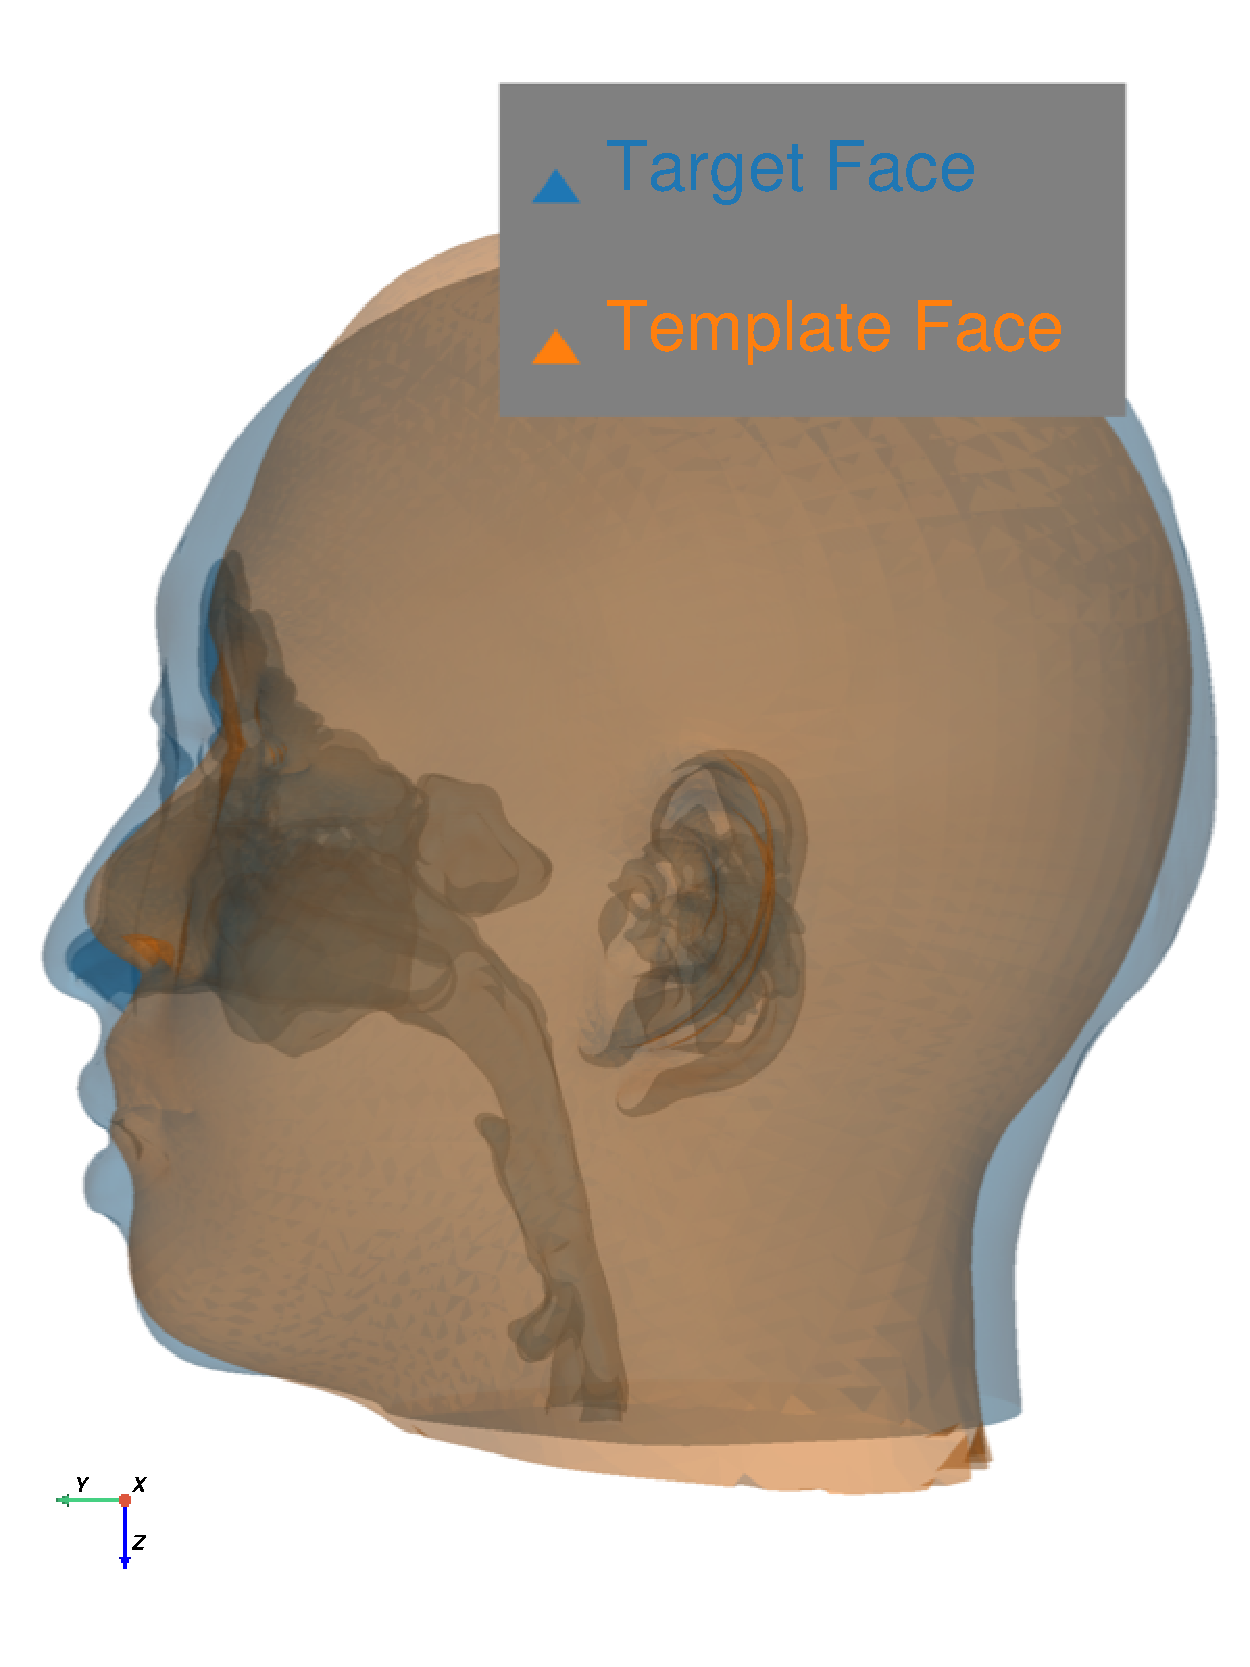
\includegraphics[height = 0.55 \linewidth]{fig/register/align-face.pdf}
    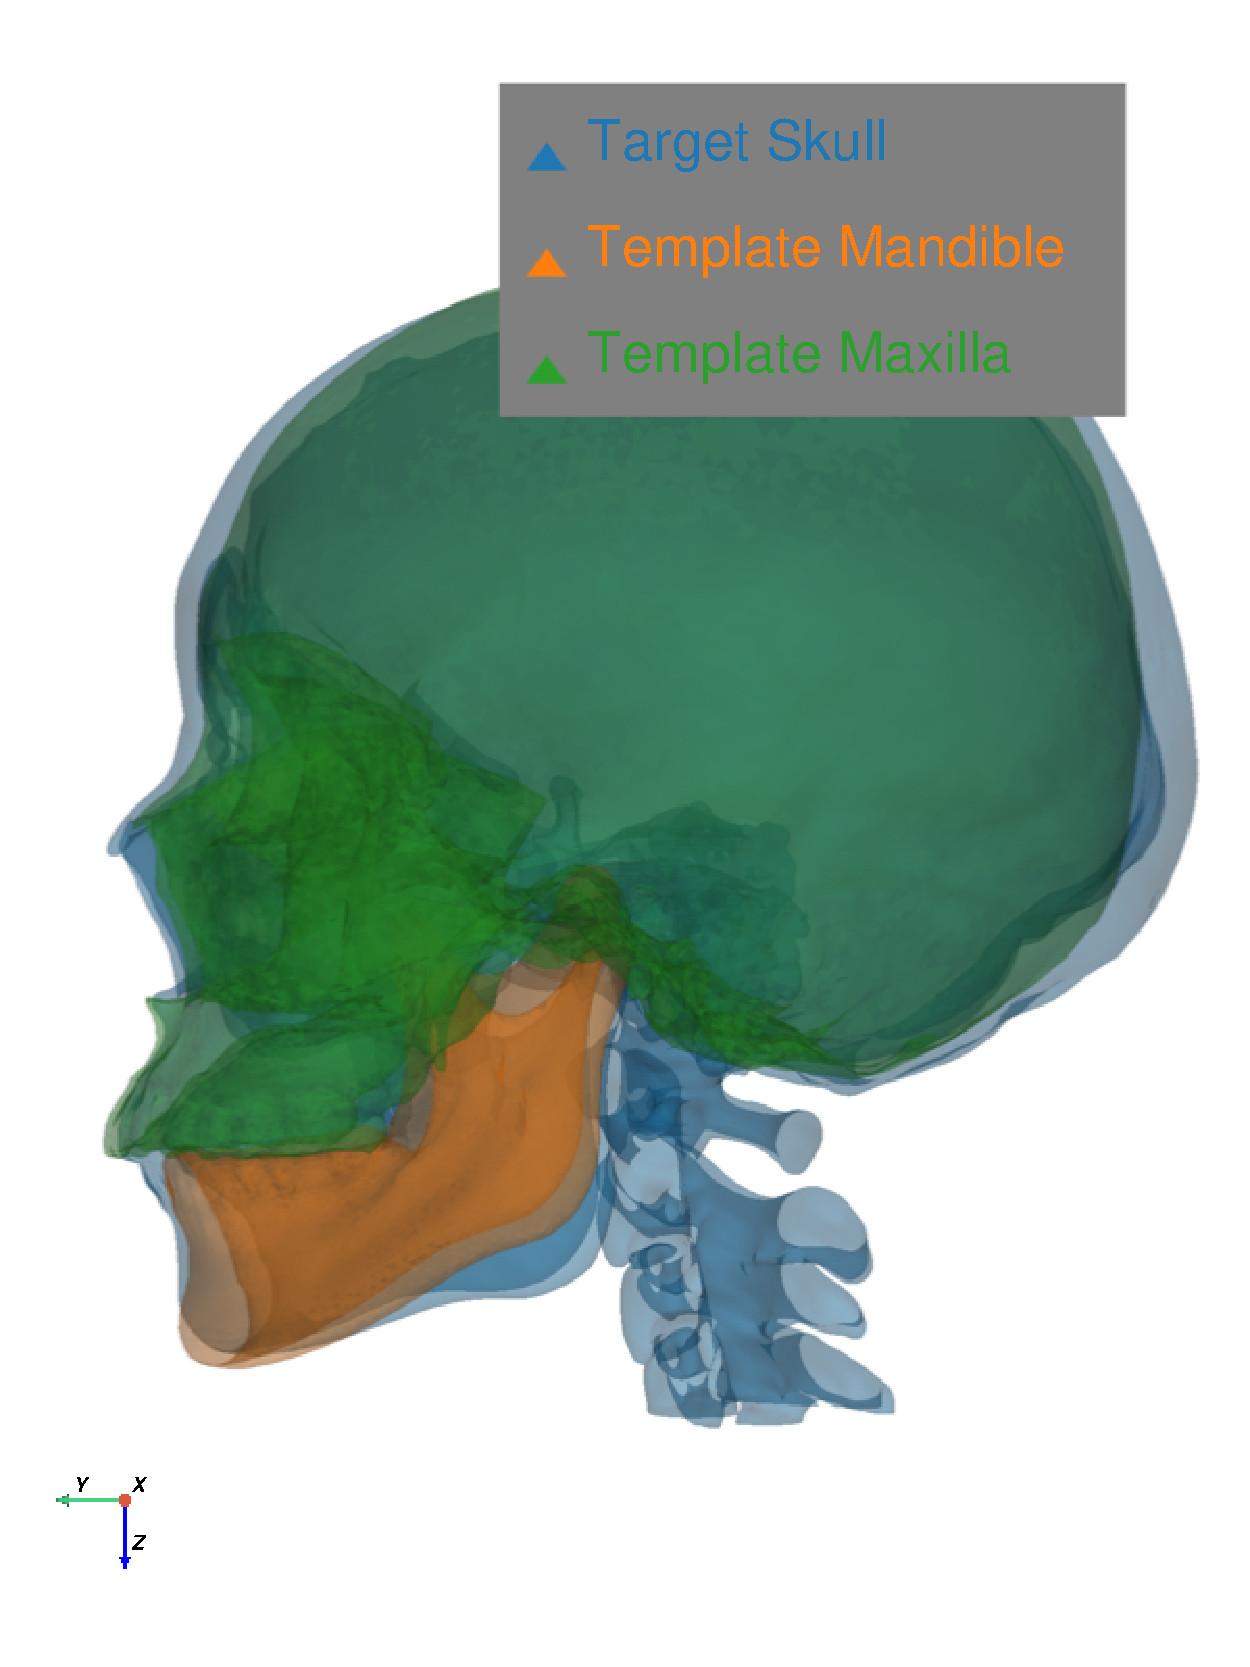
\includegraphics[height = 0.55 \linewidth]{fig/register/align-skull.pdf}
  \end{figure}
\end{frame}

\begin{frame}{非刚性配准}
  \begin{enumerate}
    \item 为每个顶点初始化仿射变换 $\vb{X}_i \in \mathbb{R}^{3 \times 4}$
    \item 对于每一组超参数 $\alpha_i, \beta_i$
          \begin{enumerate}
            \item 根据距离和法向寻找对应关系
                  \begin{equation*}
                    \mathrm{NN}(\vb{v}_i) = \arg\min_{\vb{u}_j \in \mathcal{T}_v} \norm{\vb{v}_i - \vb{u}_j} + \nu \norm{\vb{n}_i - \vb{n}_j}^2
                  \end{equation*}
            \item 最小化损失函数 $E = E_d + \alpha E_s + \beta E_l$
                  \begin{align*}
                    \text{distance} \quad E_d(\mathcal{X})  & = \sum_{\vb{v}_i \in \mathcal{S}_v} \norm{\vb{X}_i \vb{v}_i - \mathrm{NN}(\vb{X}_i \vb{v}_i)}^2 \\
                    \text{stiffness} \quad E_s(\mathcal{X}) & = \sum_{(\vb{v}_i, \vb{v}_j) \in \mathcal{E}} \norm{(\vb{X}_i - \vb{X}_j) \vb{G}}_F^2           \\
                    \text{landmarks} \quad E_l(\mathcal{X}) & = \sum_{(\vb{l}_i, \vb{v}_i) \in \mathcal{L}} \norm{\vb{X}_i \vb{v}_i - \vb{l}_i}^2
                  \end{align*}
          \end{enumerate}
  \end{enumerate}
\end{frame}

\begin{frame}{非刚性配准}
  \begin{figure}
    \centering
    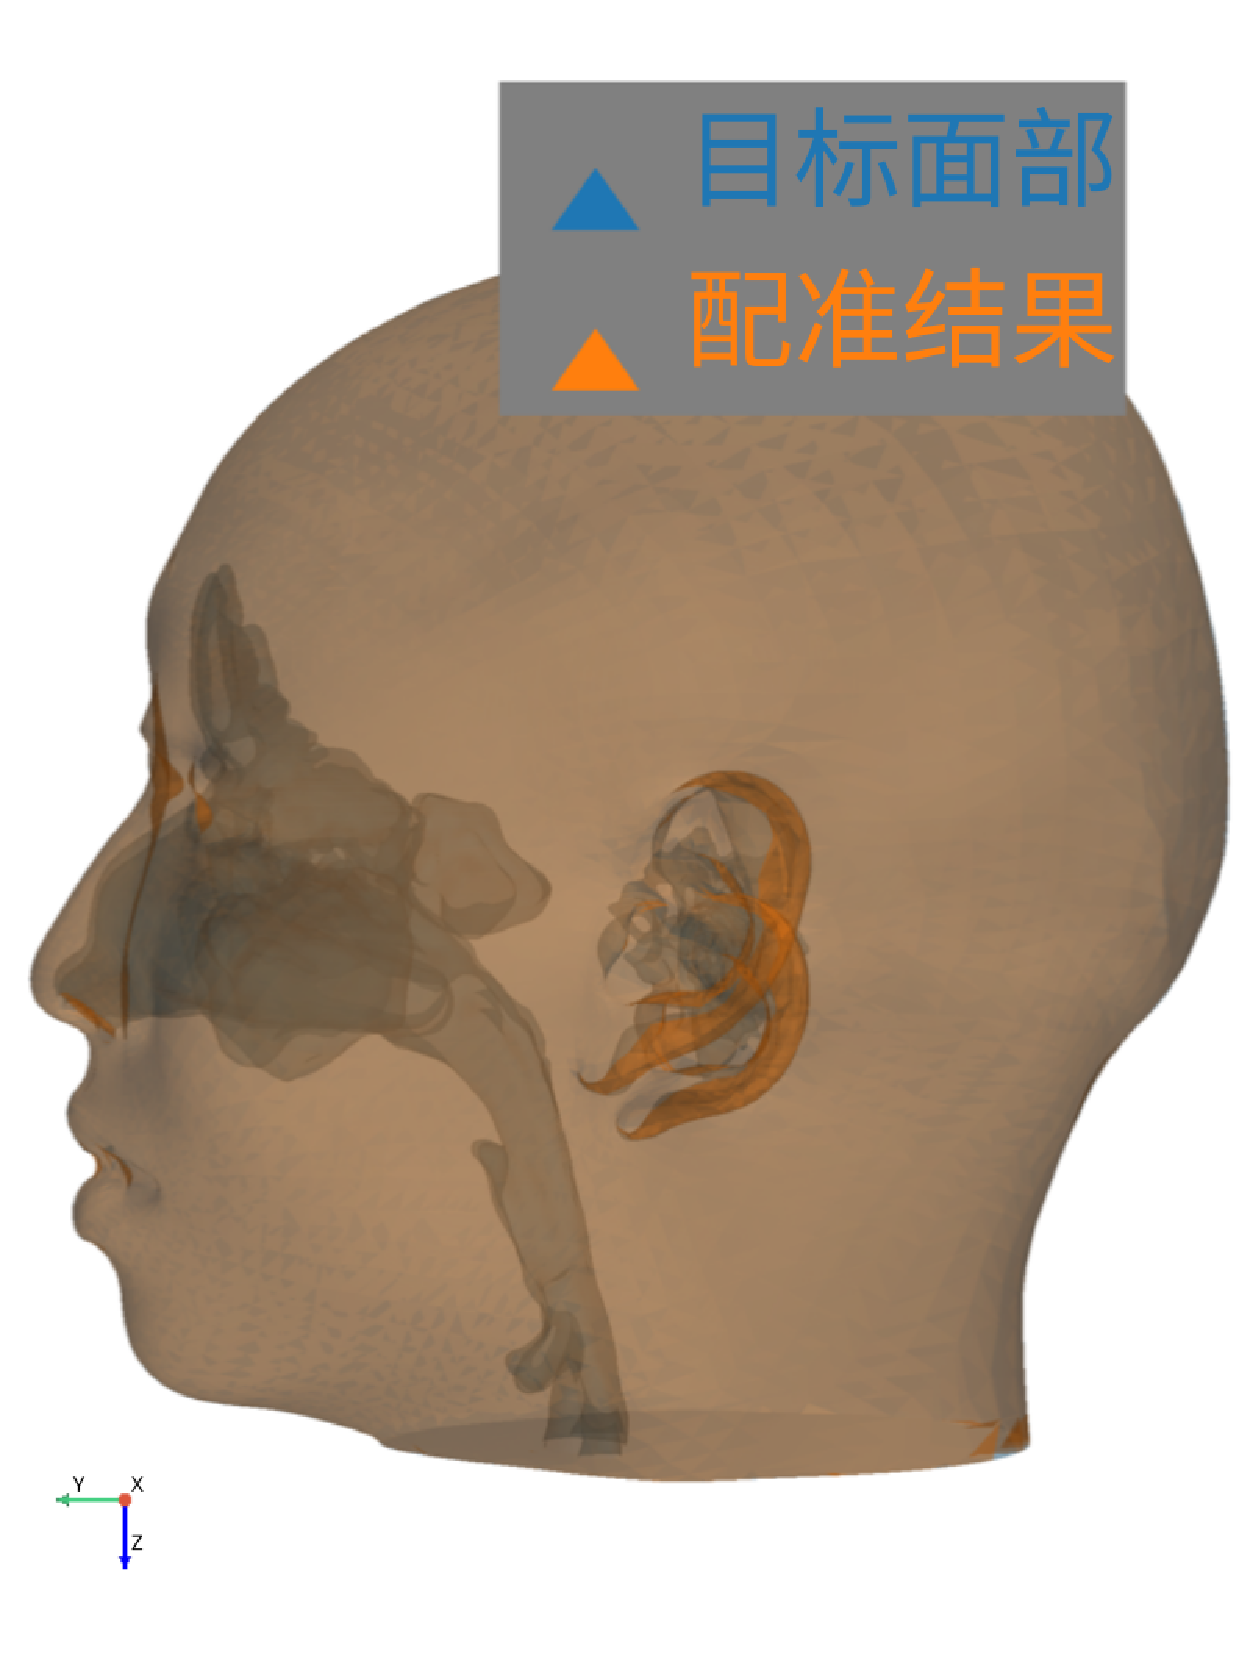
\includegraphics[height = 0.6 \linewidth]{fig/register/register-face.pdf}
    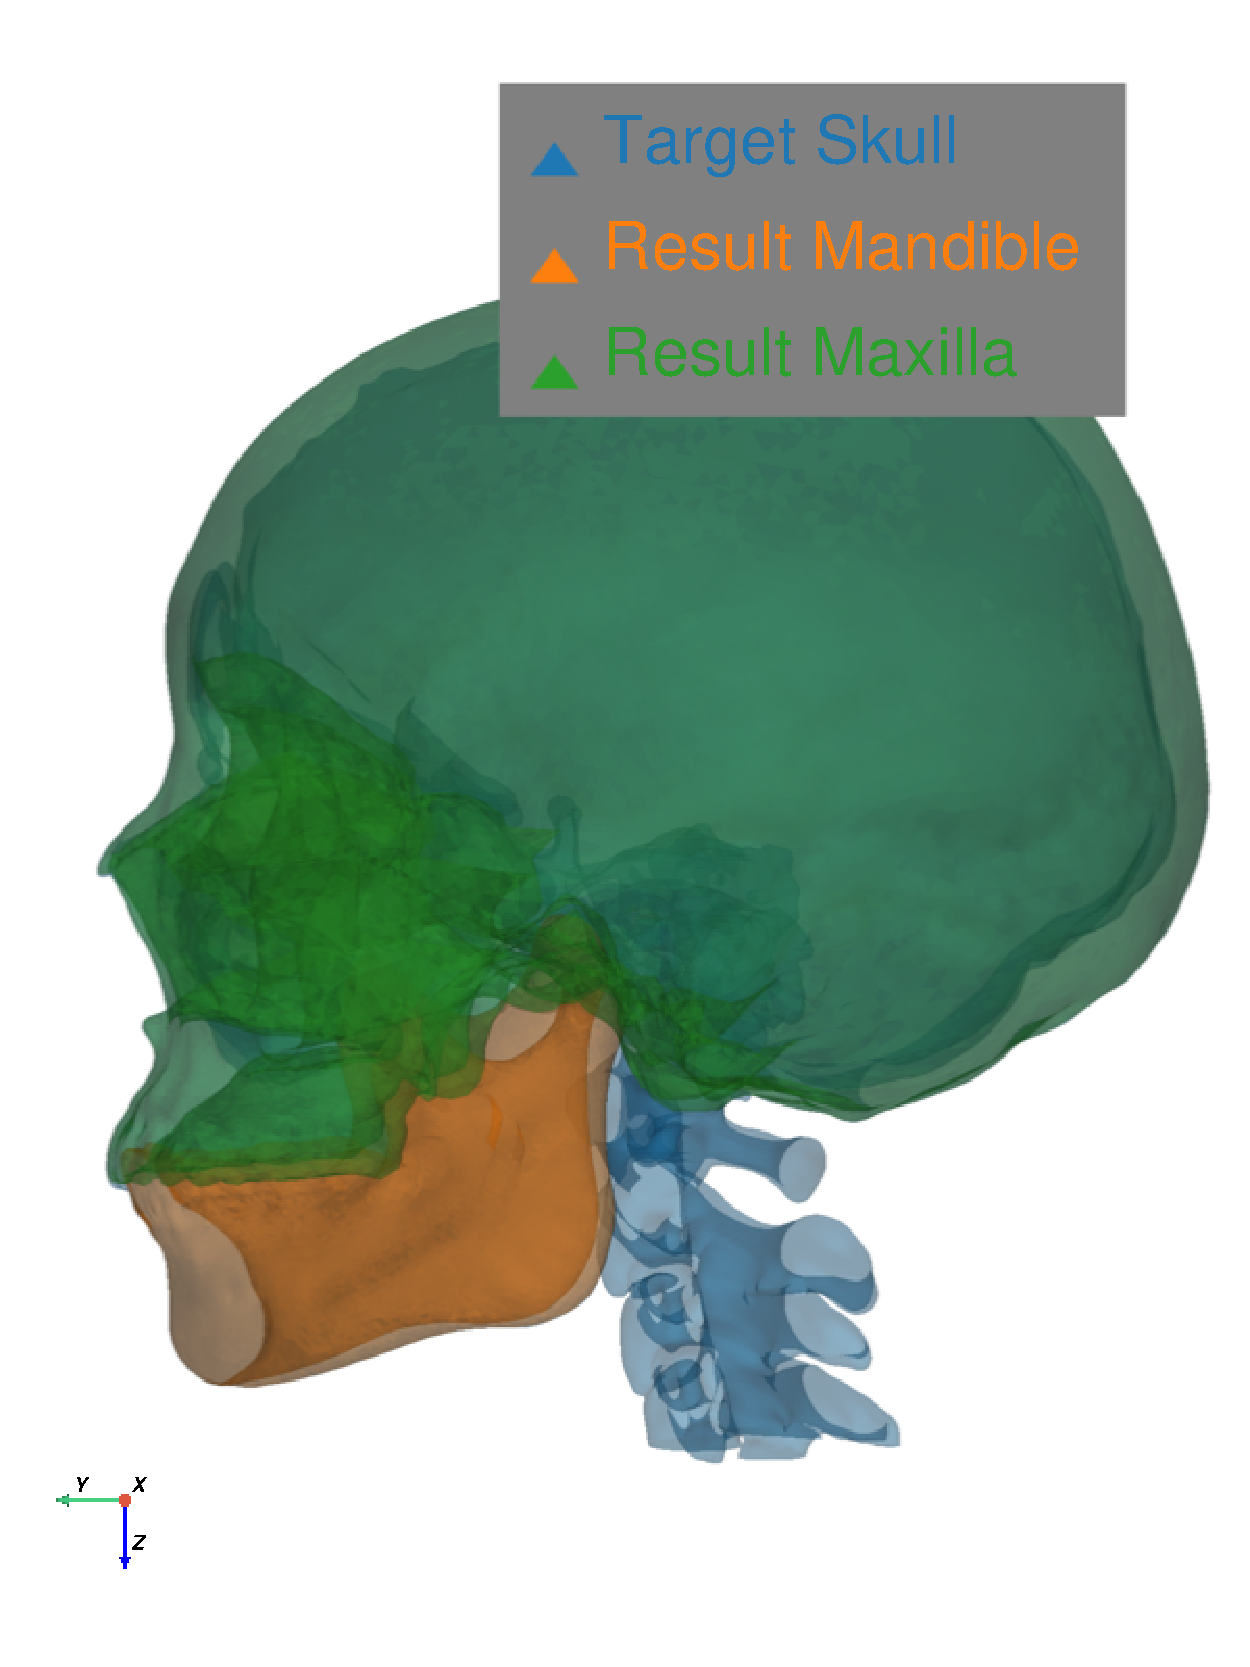
\includegraphics[height = 0.6 \linewidth]{fig/register/register-skull.pdf}
  \end{figure}
\end{frame}

\begin{frame}{四面体划分}
  % \begin{enumerate}
  %   \item 对上下颌骨应用 MeshFix 以消除自相交
  %   \item 布尔合并上下颌骨得到整体骨骼模型
  %   \item 使用 TetGen 进行四面体划分
  %   \item 根据剩余对应关系插值得到稠密的术前后骨骼位移
  % \end{enumerate}
  \begin{figure}
    \centering
    \includegraphics[height = 0.6 \linewidth]{fig/tetra.png}
  \end{figure}
\end{frame}

\section{生物力学模型}

\begin{frame}{Mass Tensor Model (MTM)}
  连续体上定义的能量 $\Longrightarrow$ 离散的四面体上力 $\bqty{\vb{f}}$ 与位移 $\bqty{\vb{u}}$ 关系
  \begin{equation*}
    \left.
    \begin{gathered}
      W(\vb{E}) = \frac{\lambda}{2} \pqty{\tr(\vb{E})}^2 + \mu \tr(\vb{E}^2) \\
      \vb{E} = \frac{1}{2} \pqty{\grad_{\vb{x}}{\vb{u}} + \pqty{\grad_{\vb{x}}{\vb{u}}}^T}               \\
      \vb{u}(\vb{x}) = \sum_{j = 0}^3 \alpha_j(\vb{x}) \vb{u}_j
    \end{gathered}
    \right\}
    \Longrightarrow[\vb{f}] = [\vb{K}] [\vb{u}]
  \end{equation*}
  \begin{multicols}{3}
    \begin{itemize}
      \item[$W$] 能量密度
      \item[$\vb{E}$] Lagrange 有限应变张量
      \item[$\vb{u}$] 位移场
      \item[$\alpha_j$] 重心坐标
      \item[$\vb{u}_j$] 顶点 $j$ 的位移
      \item[$\bqty{\vb{f}}$] 逐顶点受力
      \item[$\bqty{\vb{K}}$] 刚度矩阵
    \end{itemize}
  \end{multicols}
\end{frame}

\begin{frame}{Mass Tensor Model (MTM)}
  以四面体表示软组织, 以骨骼作为边界条件
  \begin{equation*}
    [\vb{K}] [\vb{u}] = [\vb{f}]
  \end{equation*}
  \begin{equation*}
    \begin{bmatrix}
      [\vb{K}]_{00} & [\vb{K}]_{01} \\
      [\vb{K}]_{10} & [\vb{K}]_{11}
    \end{bmatrix}
    \begin{bmatrix}
      [\vb{u}]_0 \\
      [\vb{u}]_1
    \end{bmatrix}
    =
    \begin{bmatrix}
      [\vb{f}]_0 \\
      \vb{0}
    \end{bmatrix}
    \Longrightarrow[\vb{K}]_{11} [\vb{u}]_1 = - [\vb{K}_{10}] [\vb{u}]_0
  \end{equation*}
  % \begin{multicols}{2}
  \begin{description}
    \item[$\vb{K}$] 刚度矩阵
    \item[$\bqty{\vb{u}}_0$] (已知) 固定顶点的位移 (紧邻骨骼)
    \item[$\bqty{\vb{u}}_1$] (待解) 自由顶点的位移 \\
          (不与骨骼直接相邻的软组织及表面)
    \item[$\bqty{\vb{f}}_1 = \bm{0}$] 平衡状态下自由顶点所受合力为零
  \end{description}
  % \end{multicols}
\end{frame}

\section{结果展示}

\begin{frame}{结果展示 > 术前}
  \begin{figure}
    \centering
    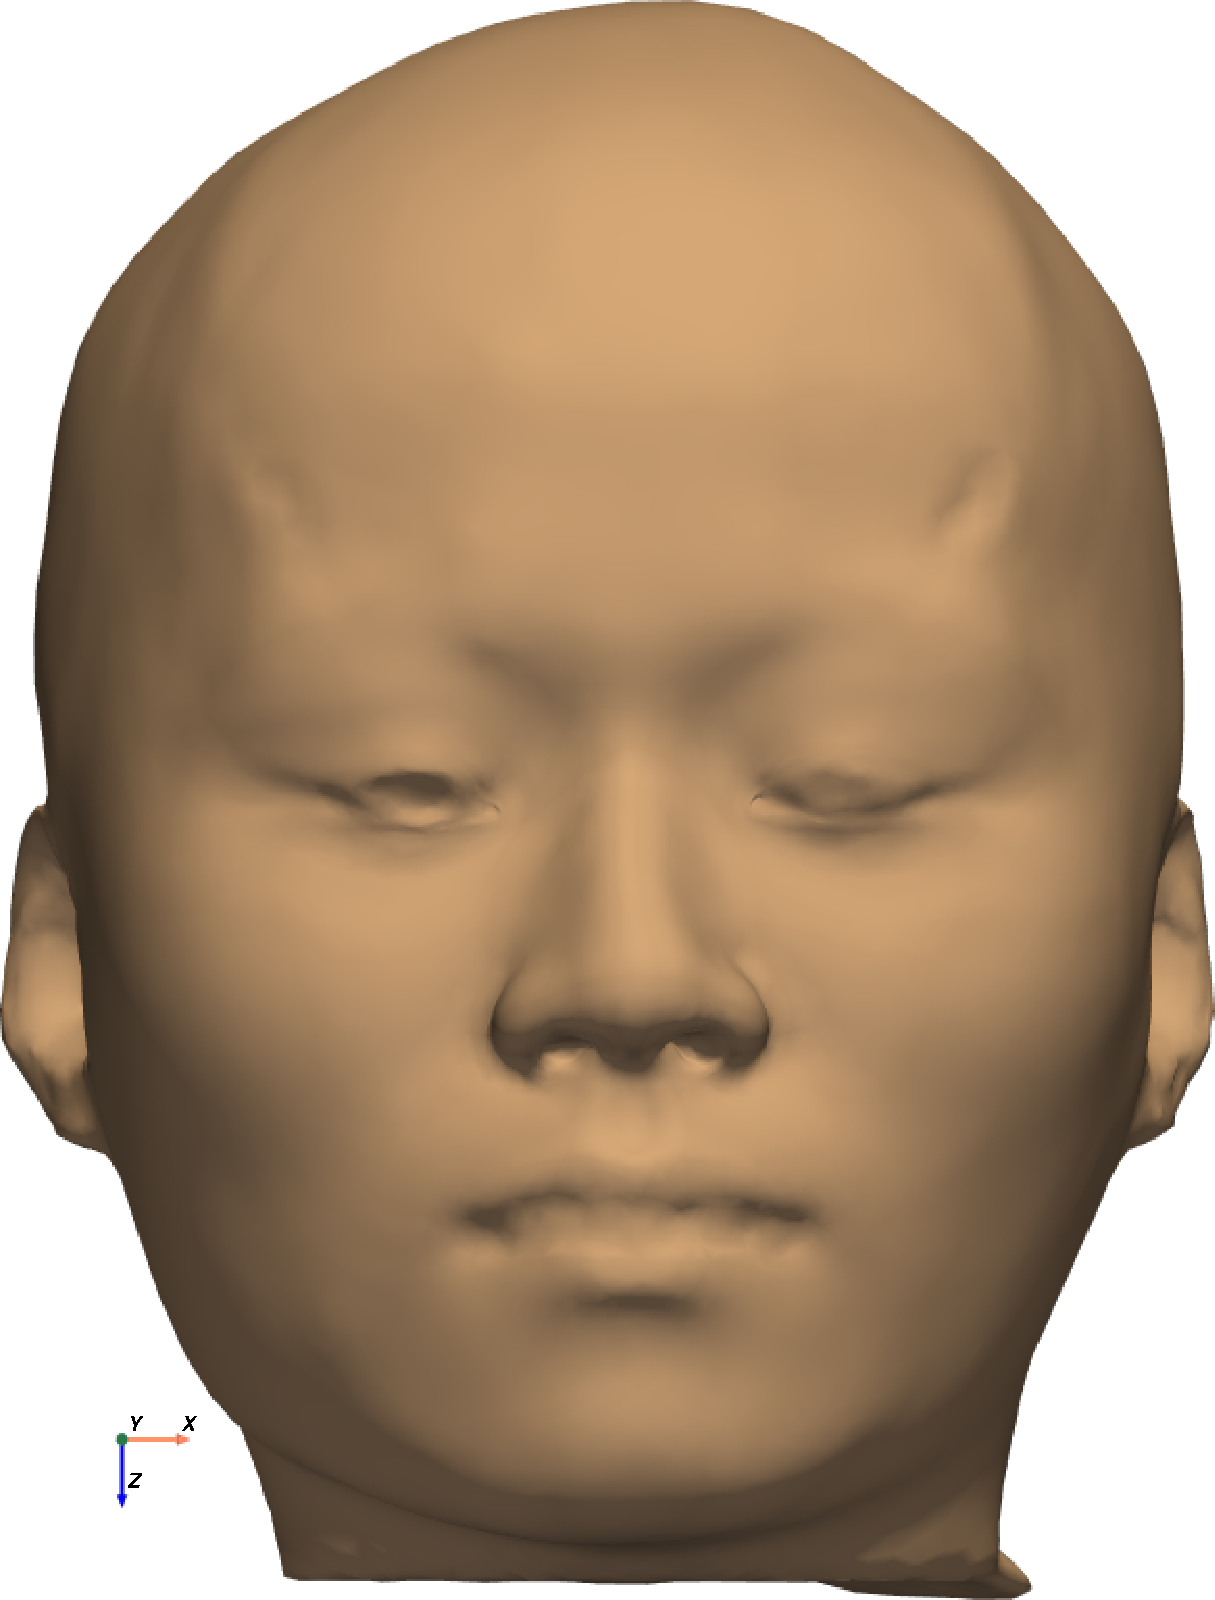
\includegraphics[height = 0.32 \linewidth]{fig/results/120056/pre-face-front.pdf}
    \includegraphics[height = 0.32 \linewidth]{fig/results/120056/pre-face-lateral.pdf}
    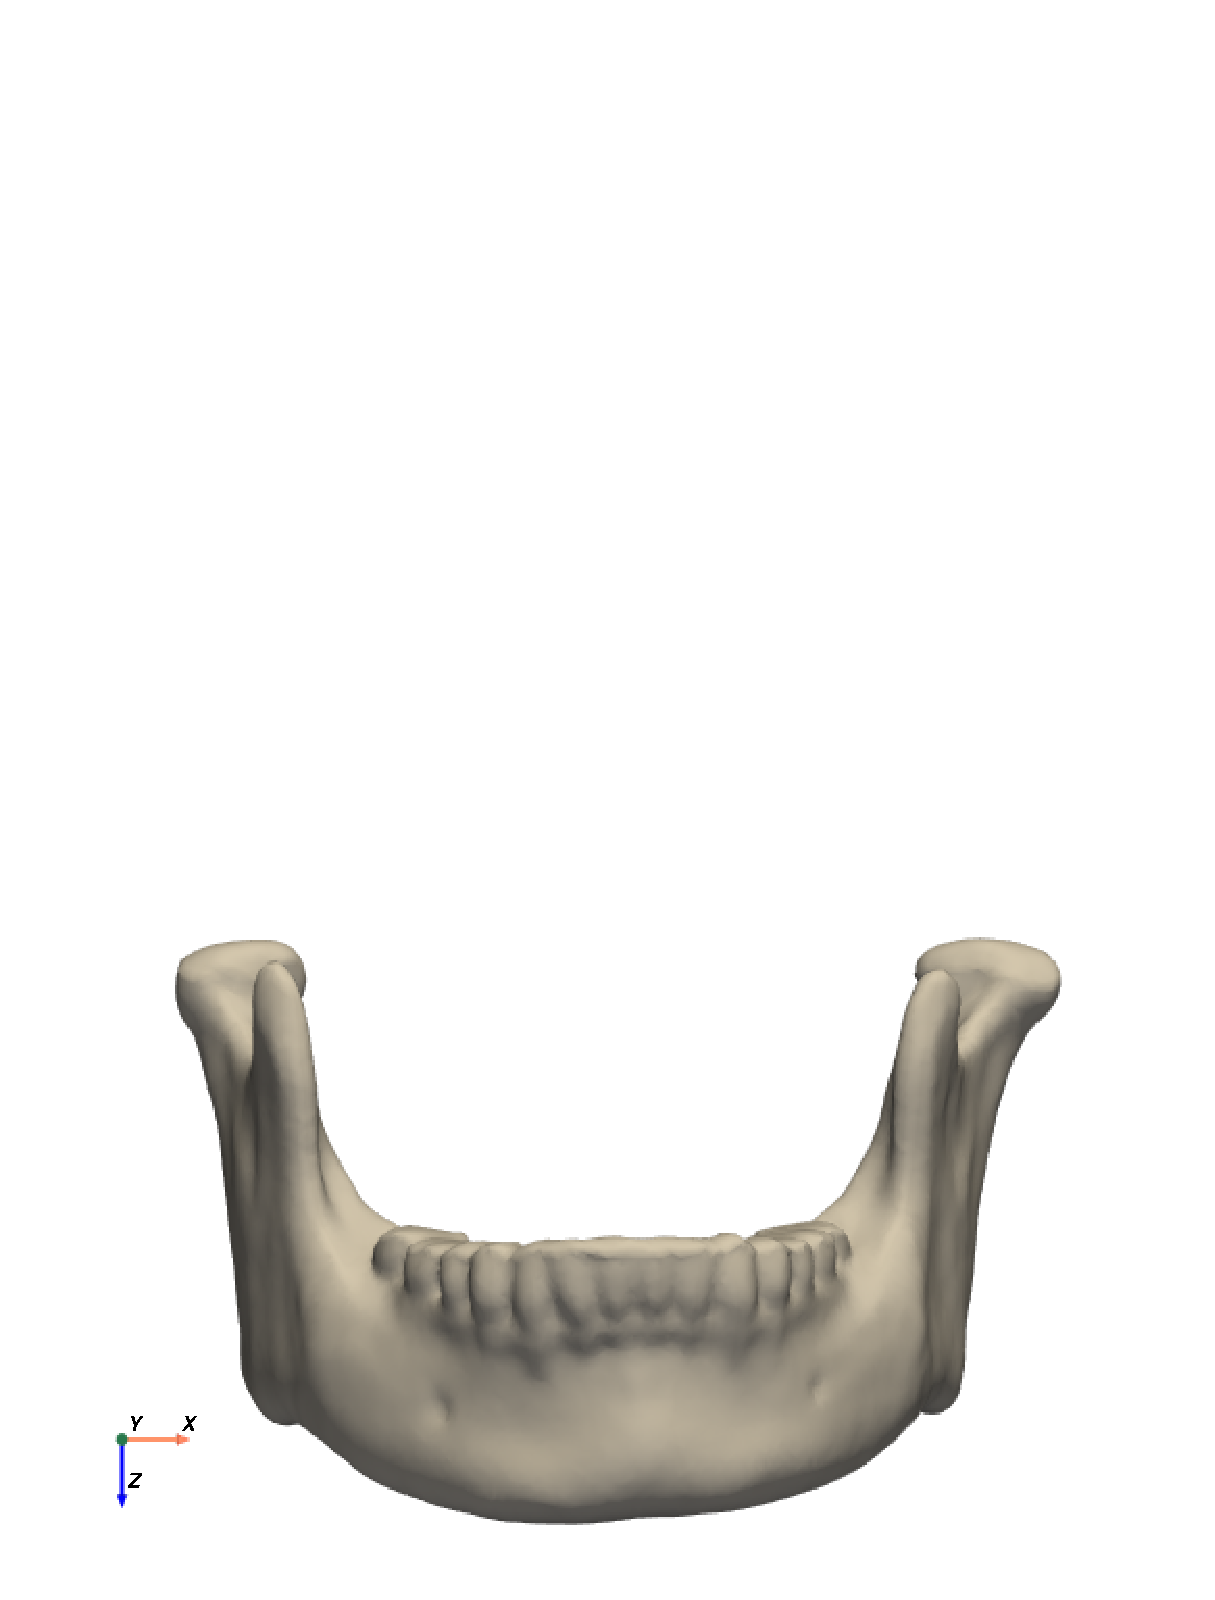
\includegraphics[height = 0.32 \linewidth]{fig/results/120056/pre-skull-front.pdf}
    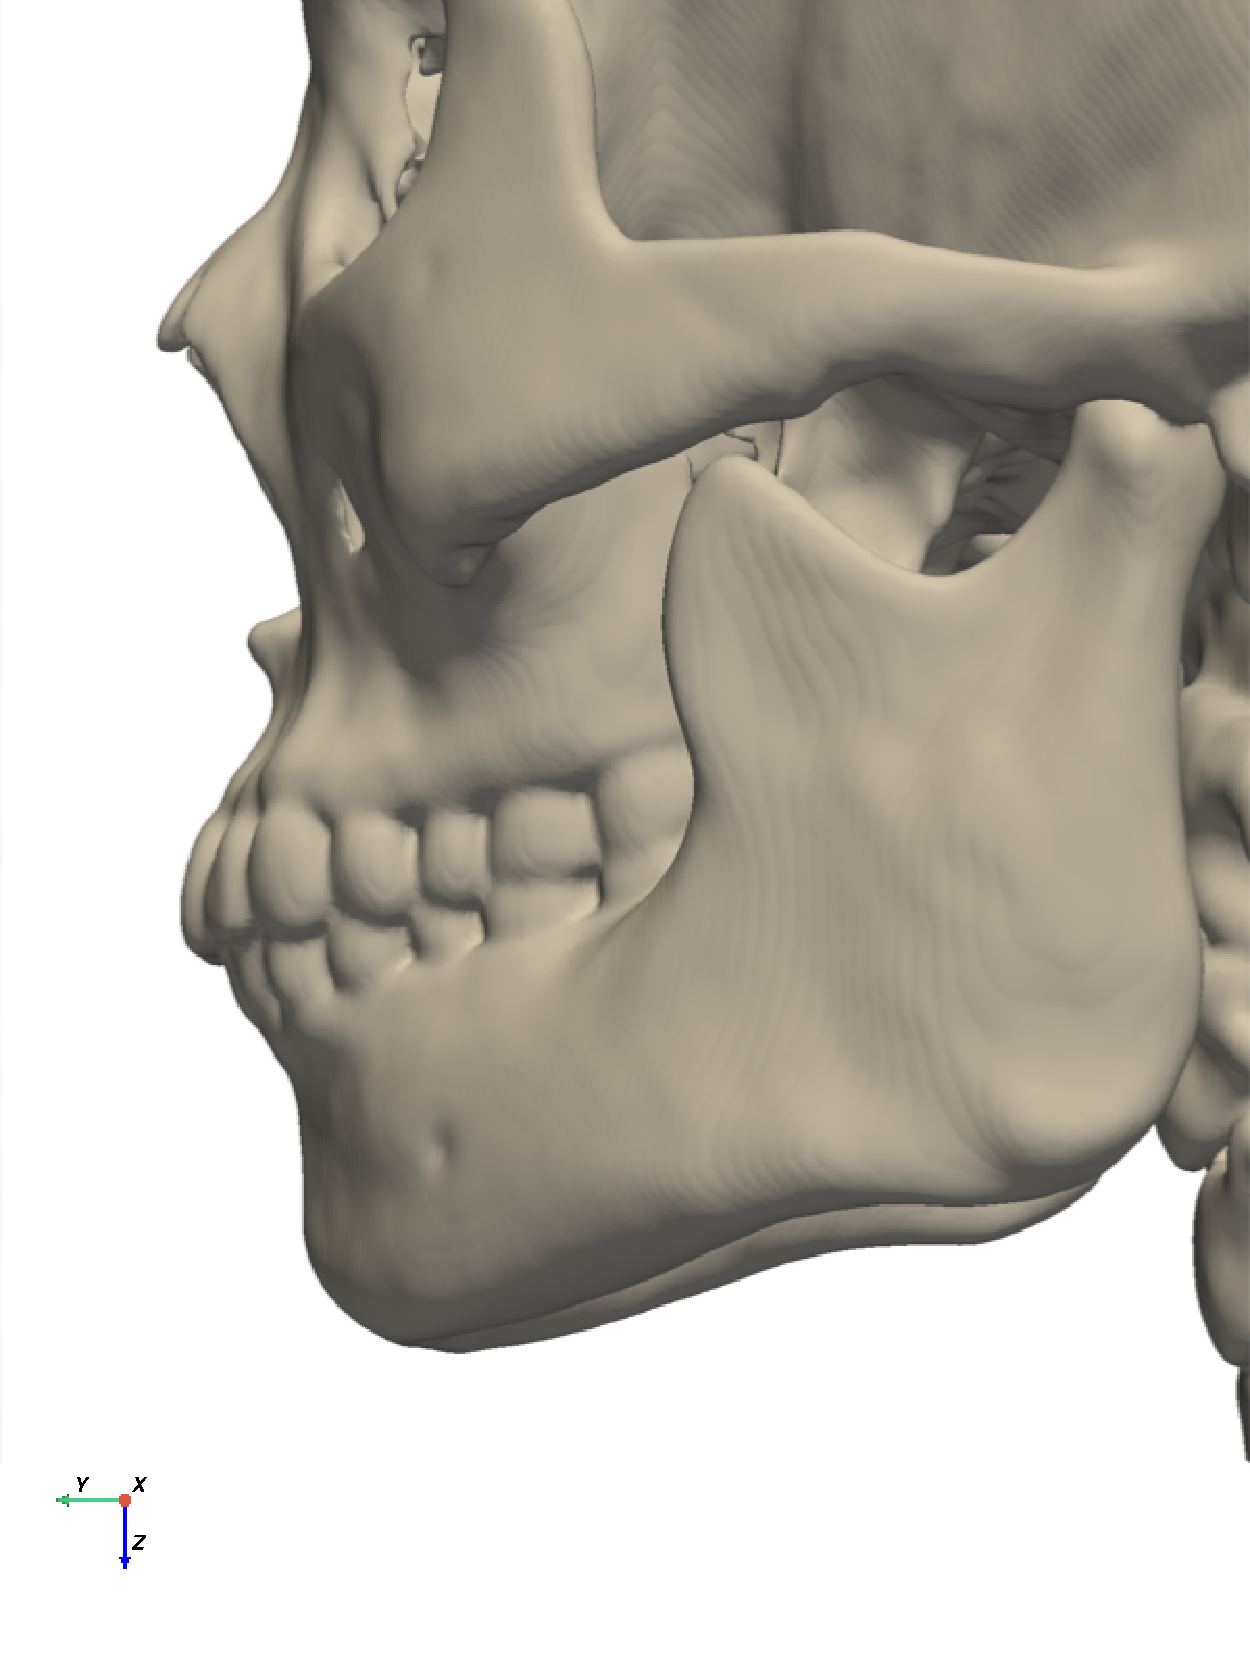
\includegraphics[height = 0.32 \linewidth]{fig/results/120056/pre-skull-lateral.pdf}
  \end{figure}
\end{frame}

\begin{frame}{结果展示 > 术后预测}
  \begin{figure}
    \centering
    \includegraphics[height = 0.32 \linewidth]{fig/results/120056/predict-front.pdf}
    \includegraphics[height = 0.32 \linewidth]{fig/results/120056/predict-lateral.pdf}
    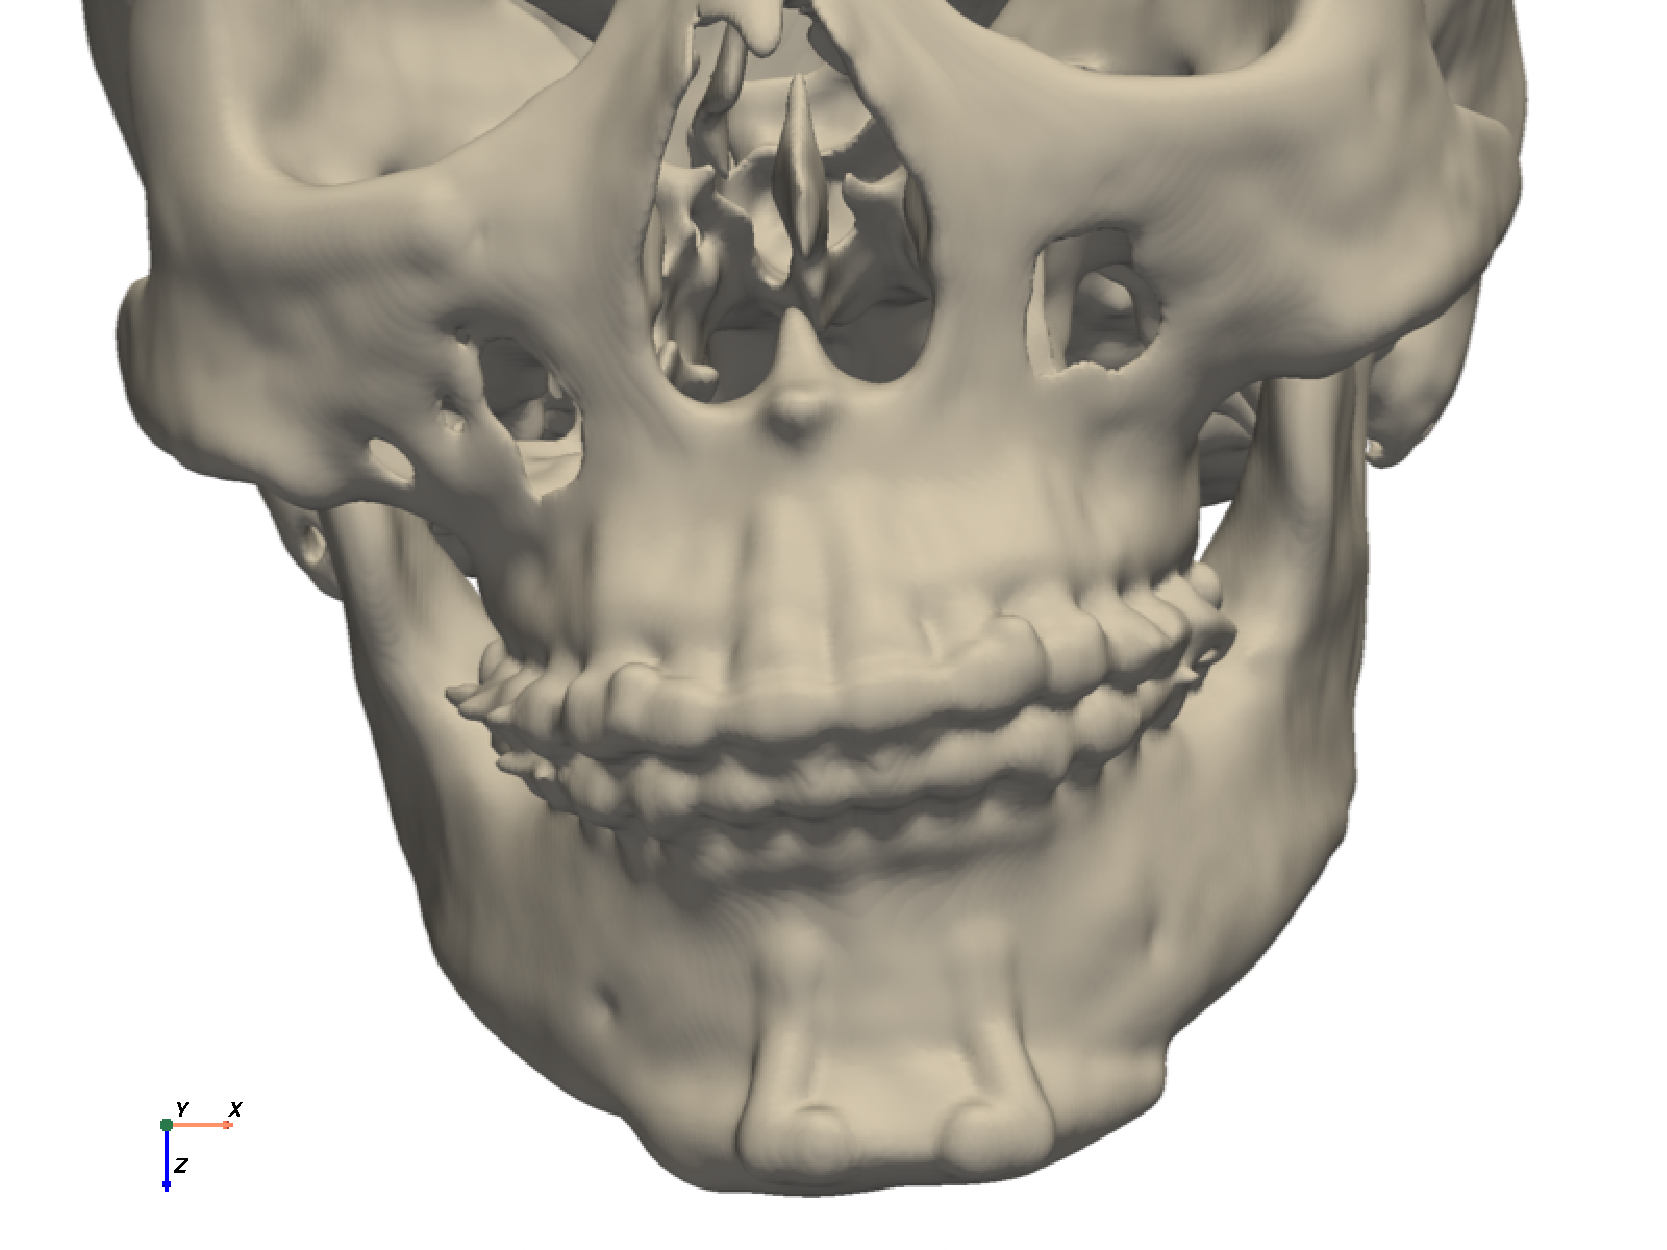
\includegraphics[height = 0.32 \linewidth]{fig/results/120056/post-skull-front.pdf}
    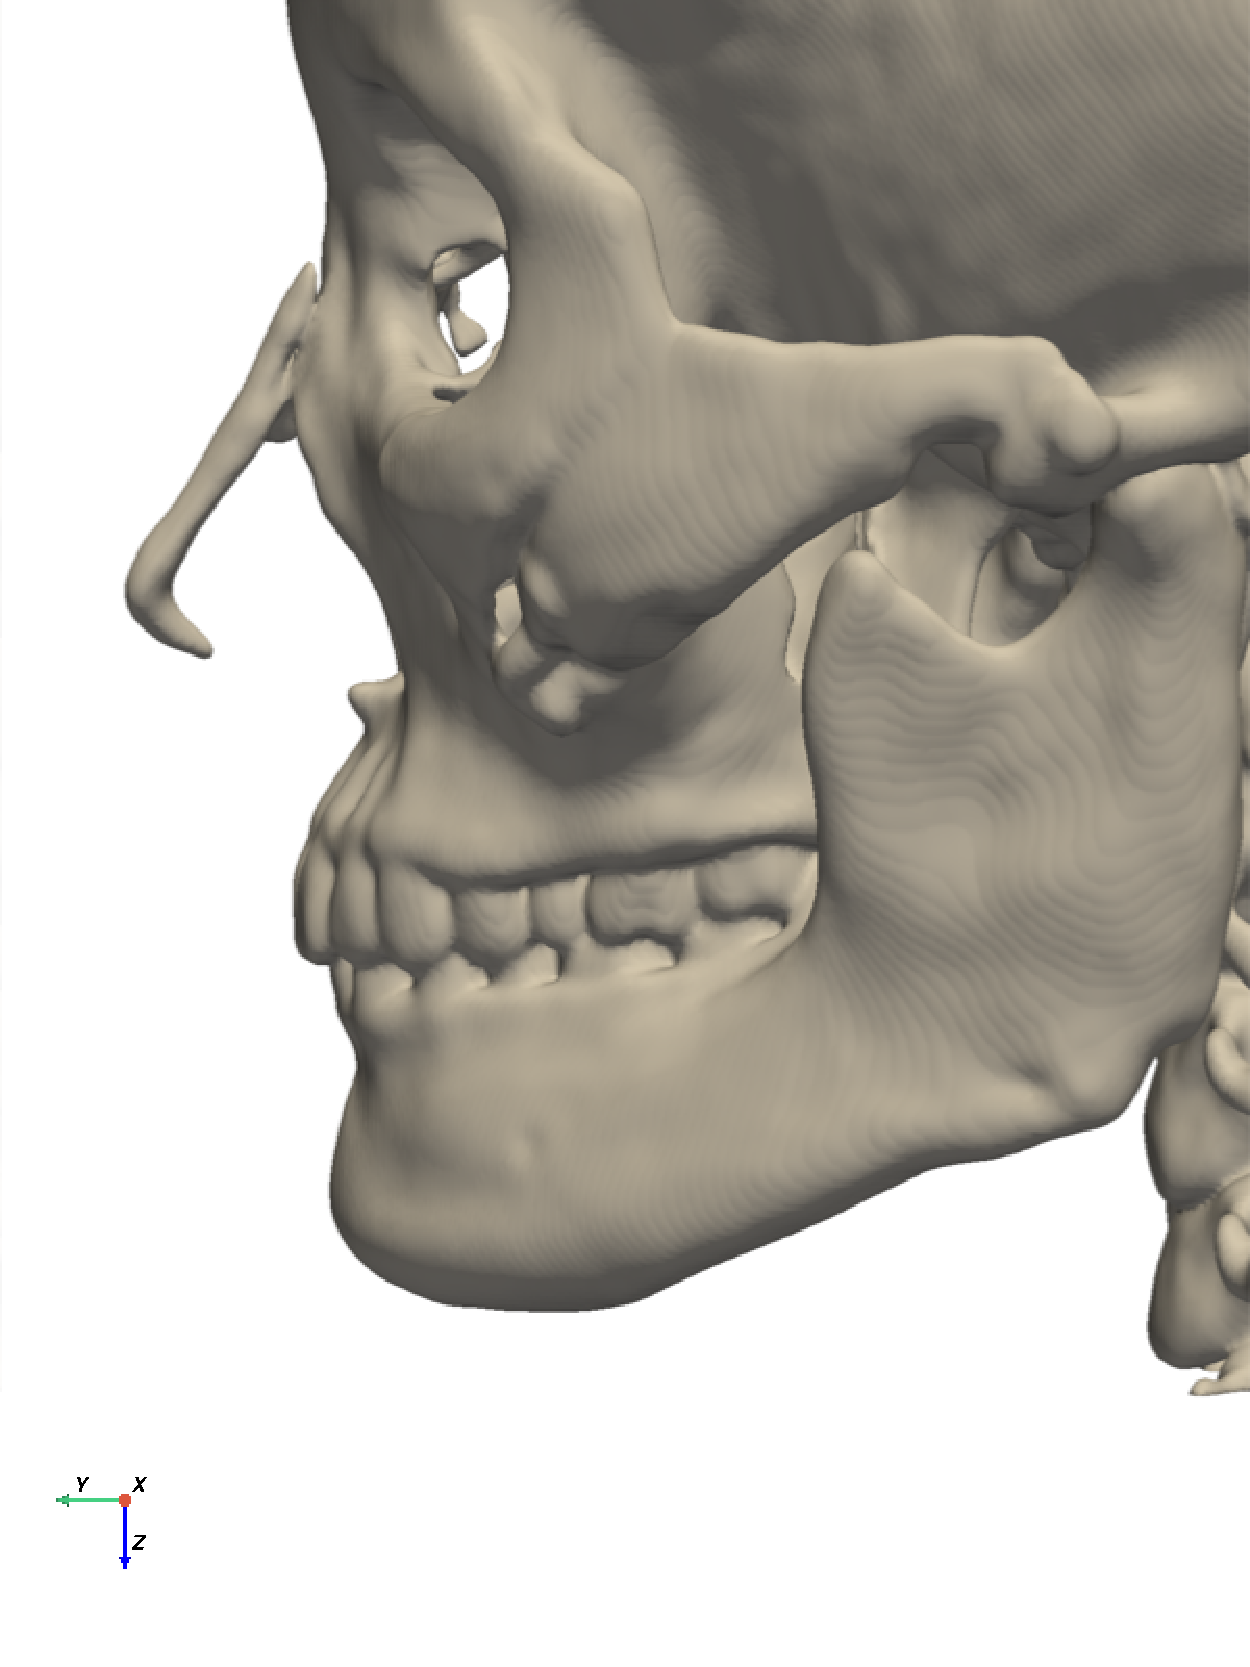
\includegraphics[height = 0.32 \linewidth]{fig/results/120056/post-skull-lateral.pdf}
  \end{figure}
\end{frame}

\begin{frame}{结果展示 > 术后实际}
  \begin{figure}
    \centering
    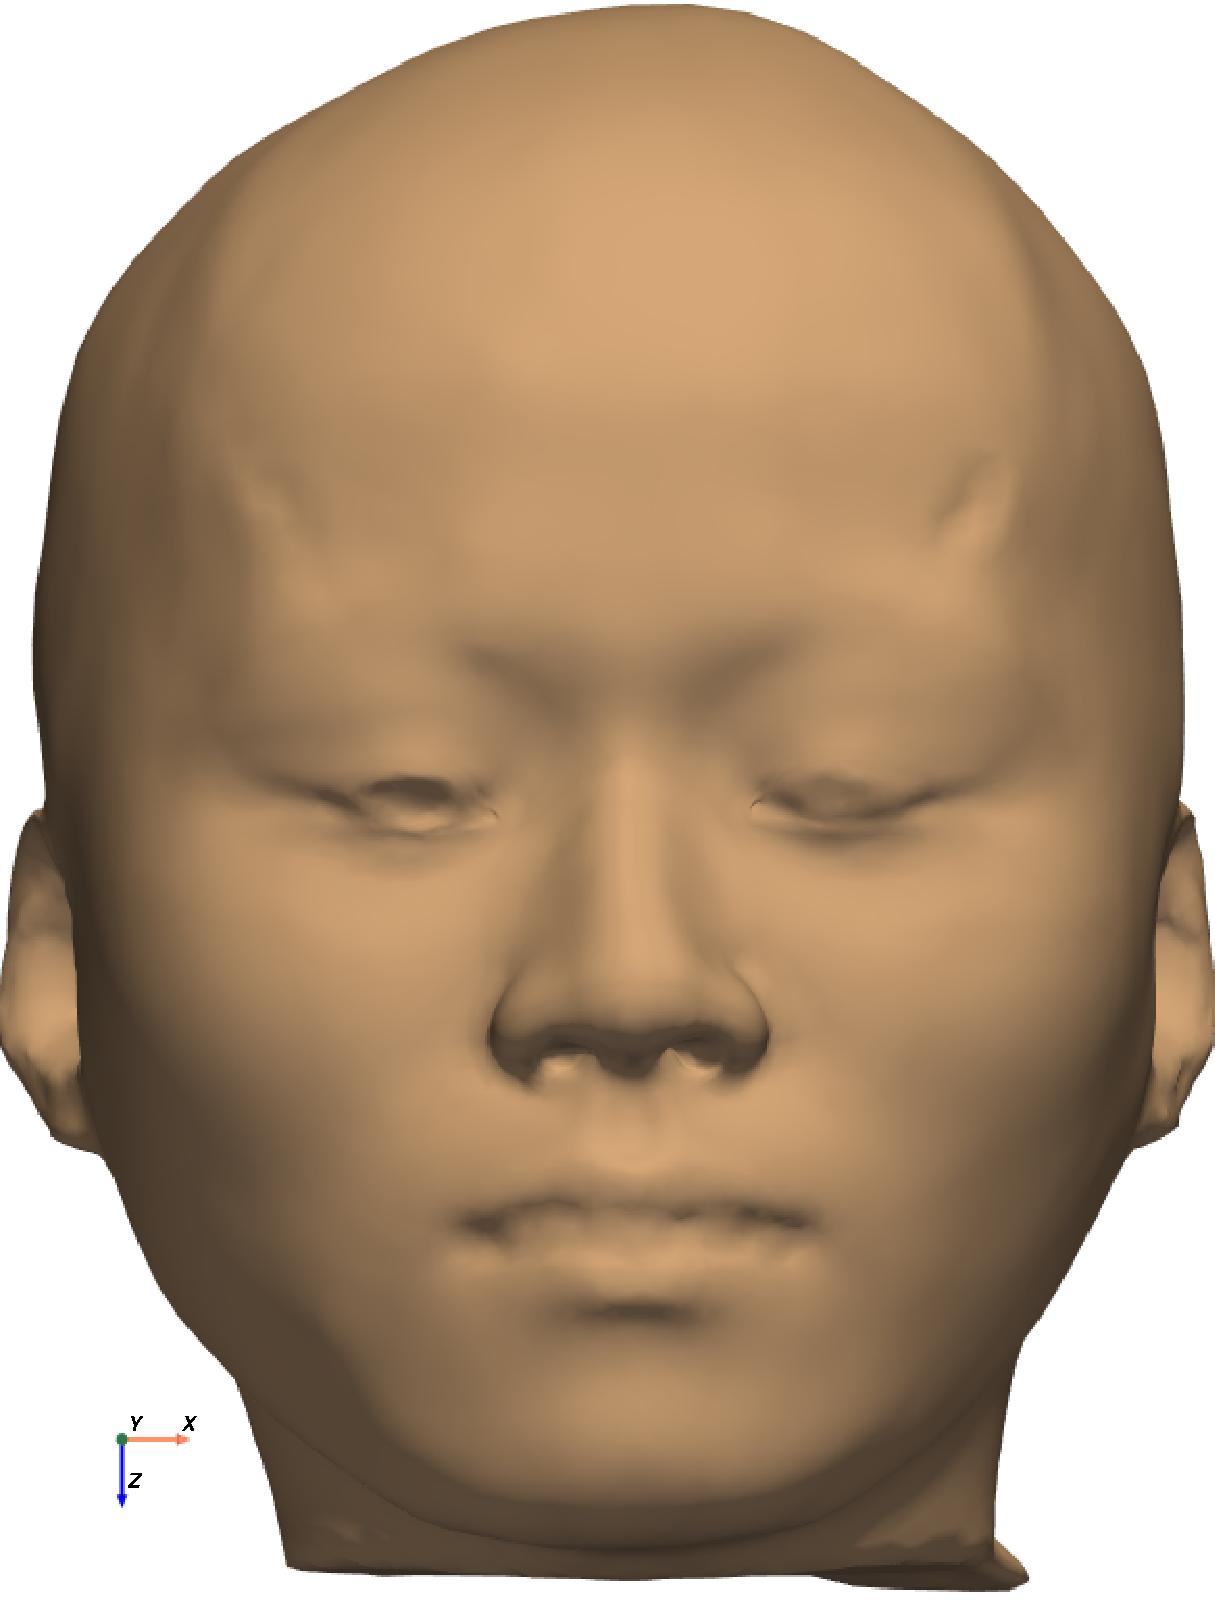
\includegraphics[height = 0.32 \linewidth]{fig/results/120056/post-face-front.pdf}
    \includegraphics[height = 0.32 \linewidth]{fig/results/120056/post-face-lateral.pdf}
    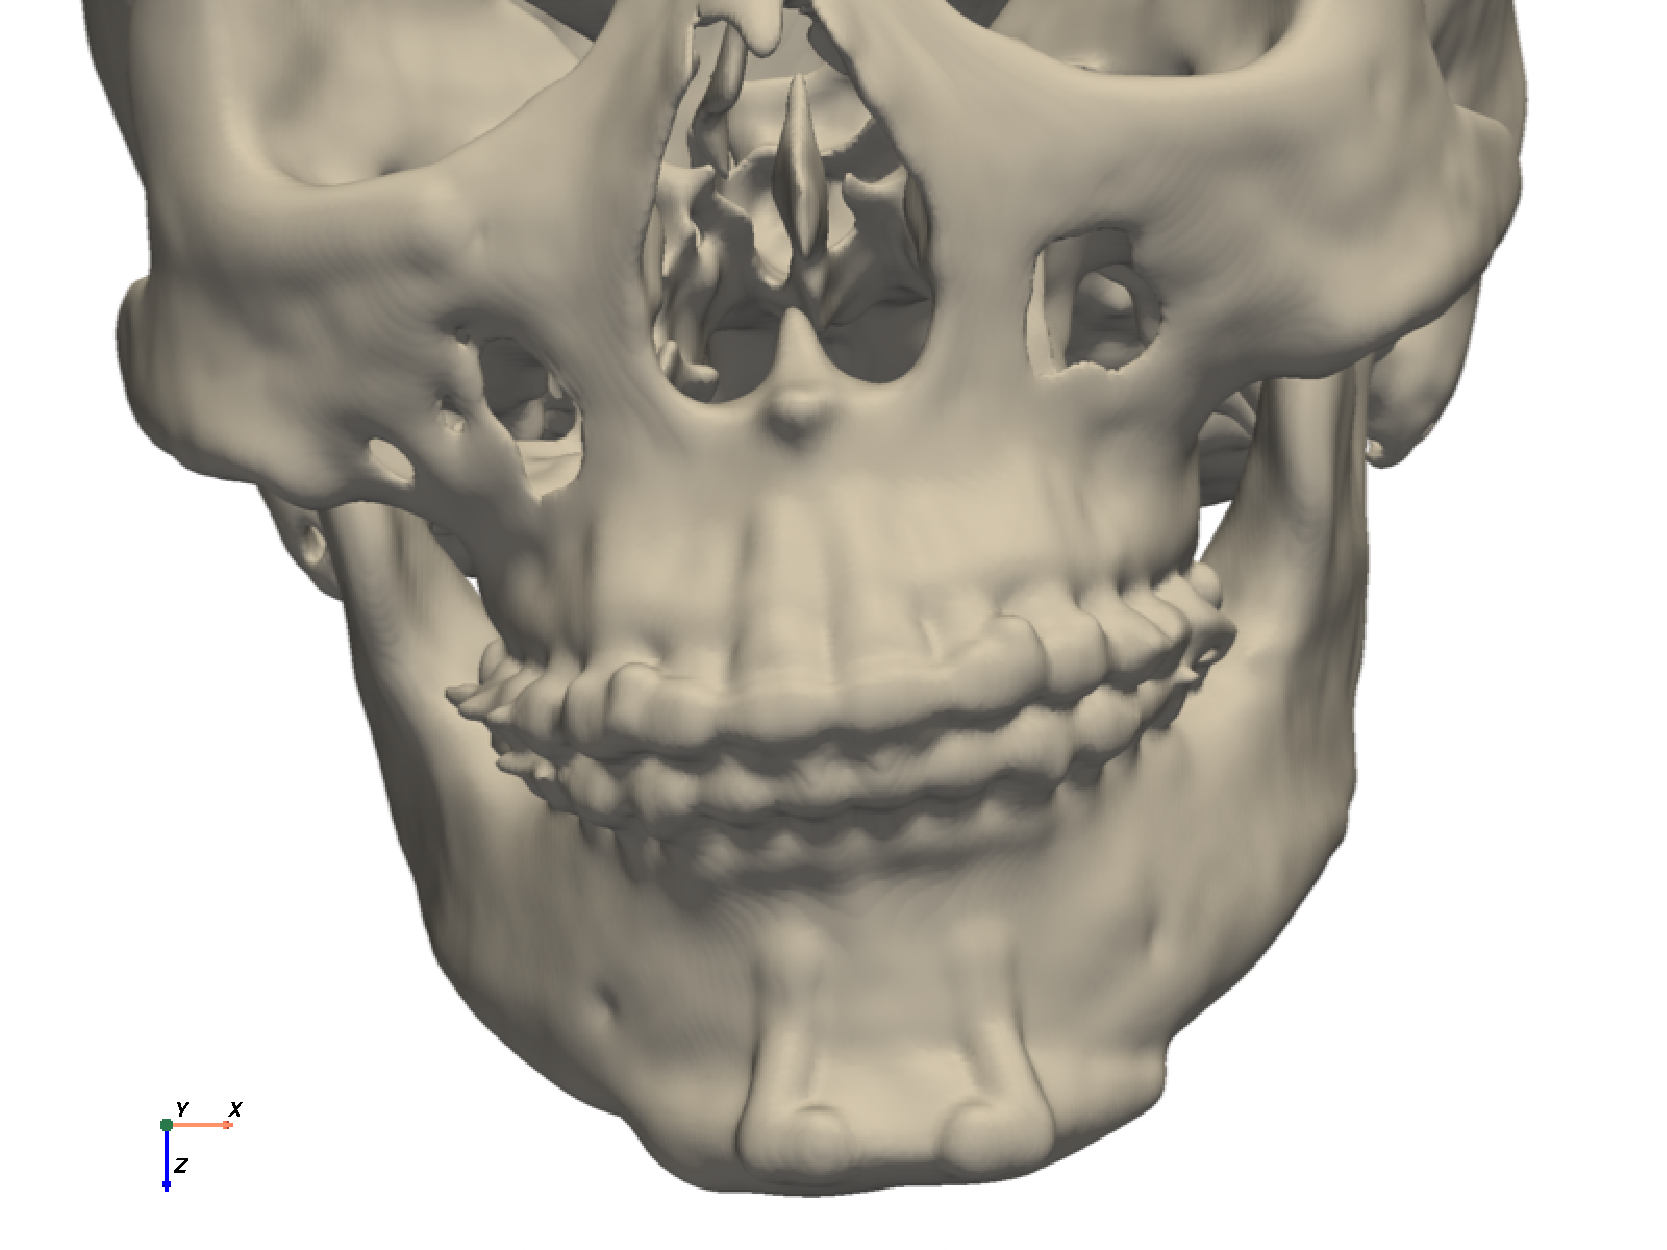
\includegraphics[height = 0.32 \linewidth]{fig/results/120056/post-skull-front.pdf}
    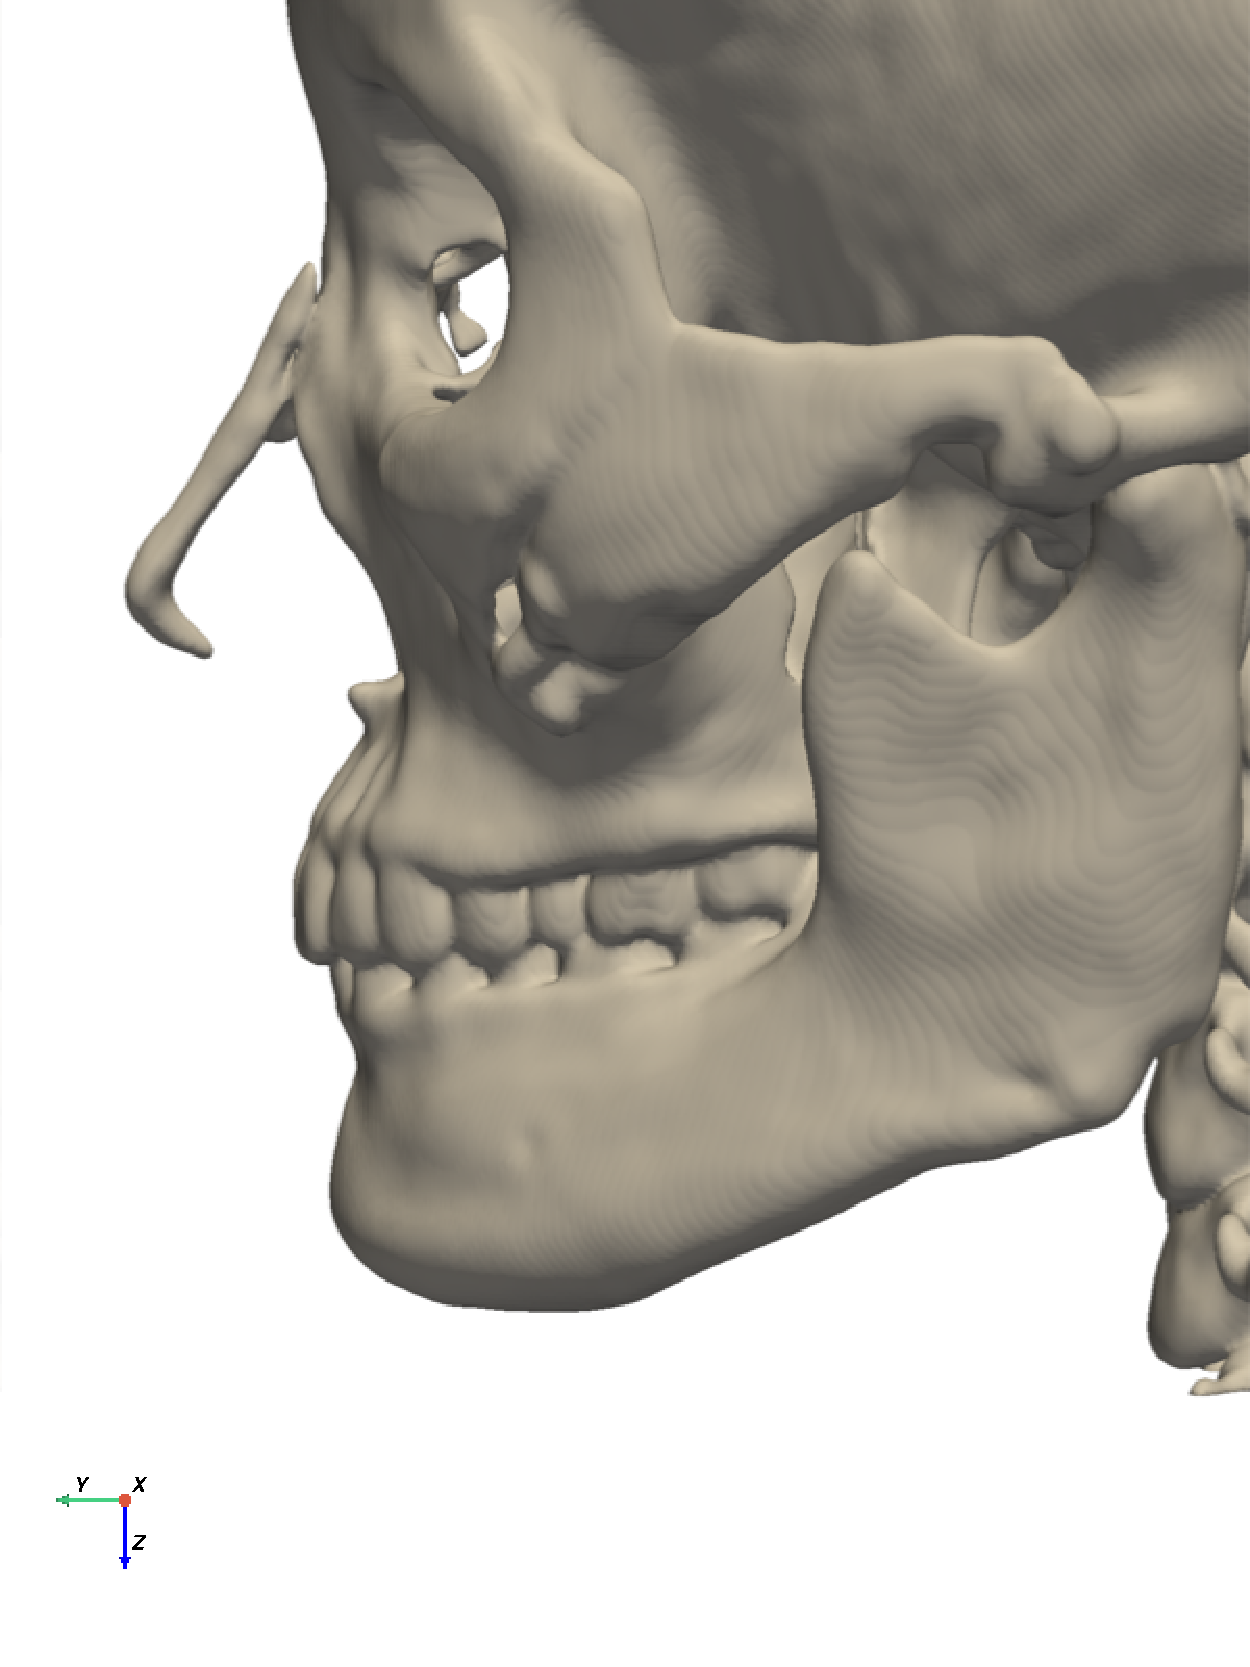
\includegraphics[height = 0.32 \linewidth]{fig/results/120056/post-skull-lateral.pdf}
  \end{figure}
\end{frame}

\begin{frame}{结果展示}
  \begin{figure}
    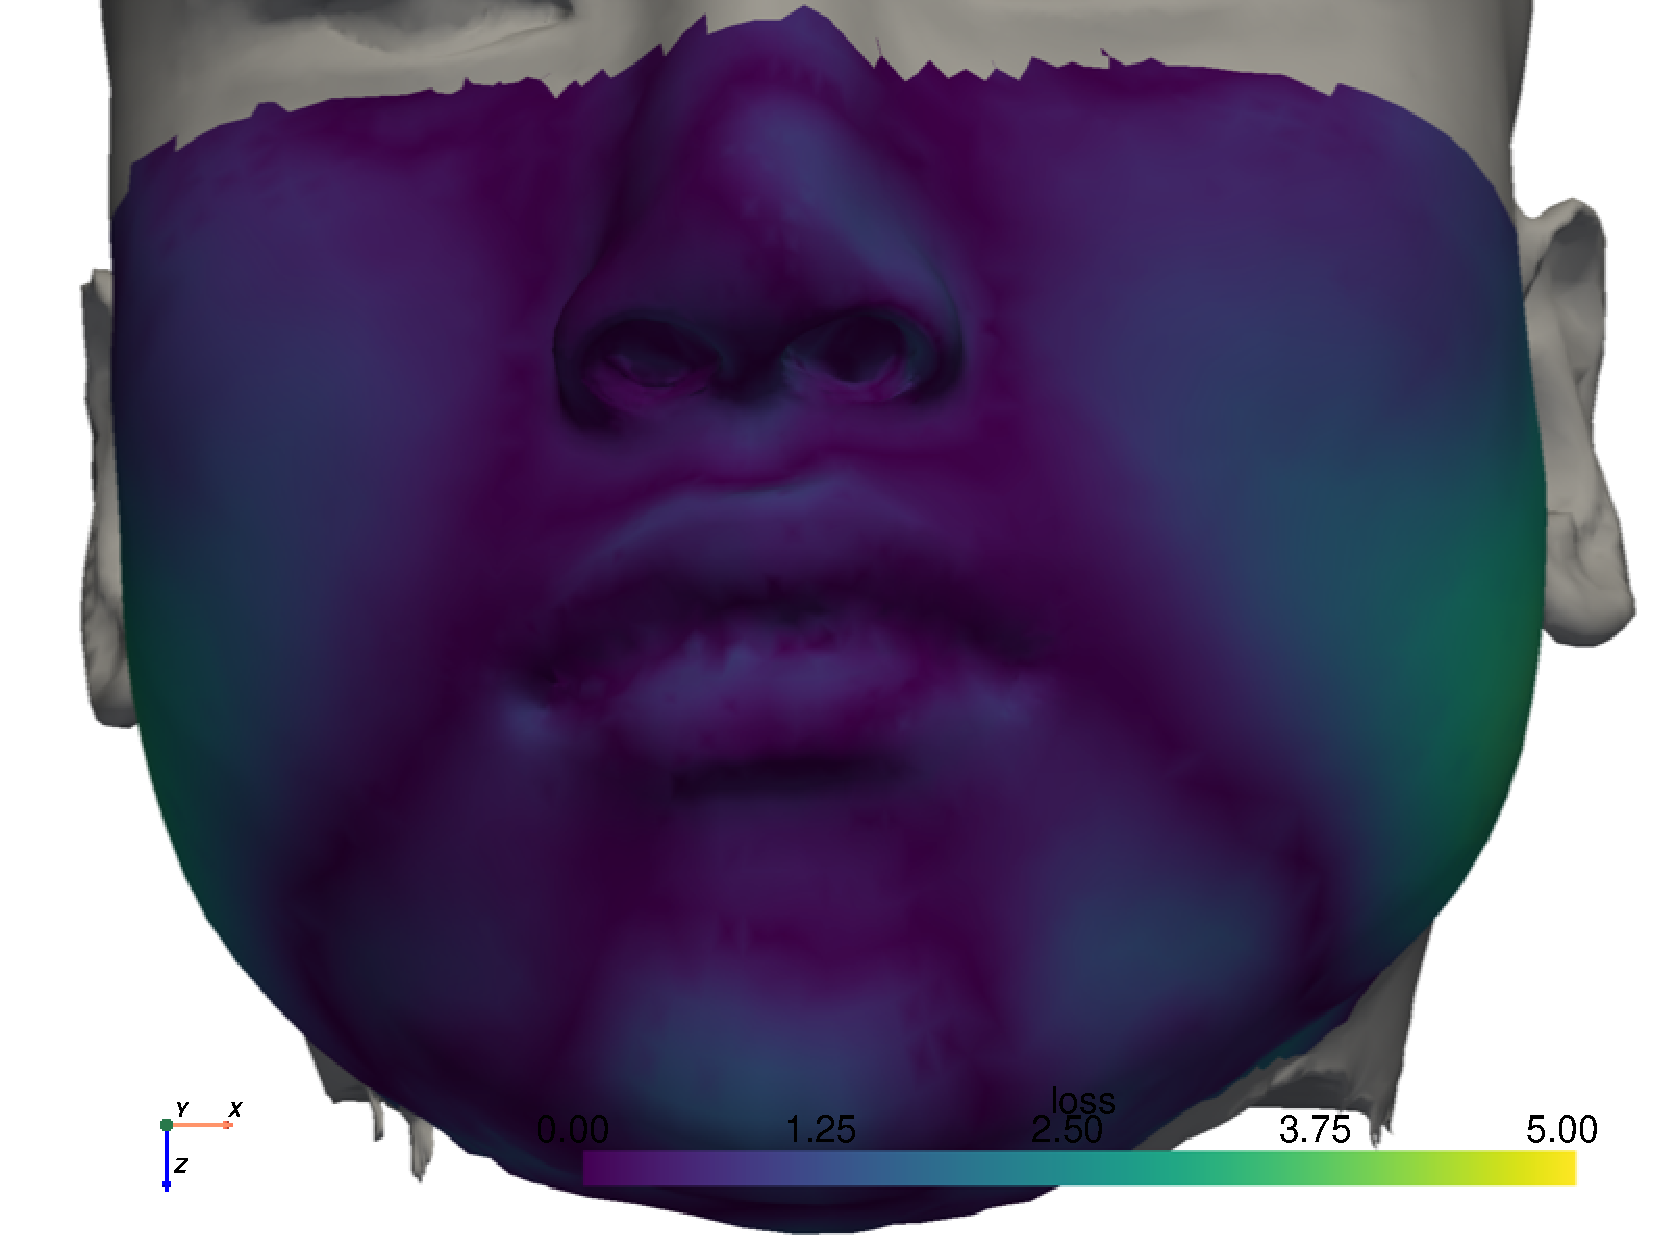
\includegraphics[height = 0.24 \linewidth]{fig/loss/111188.pdf}
    % 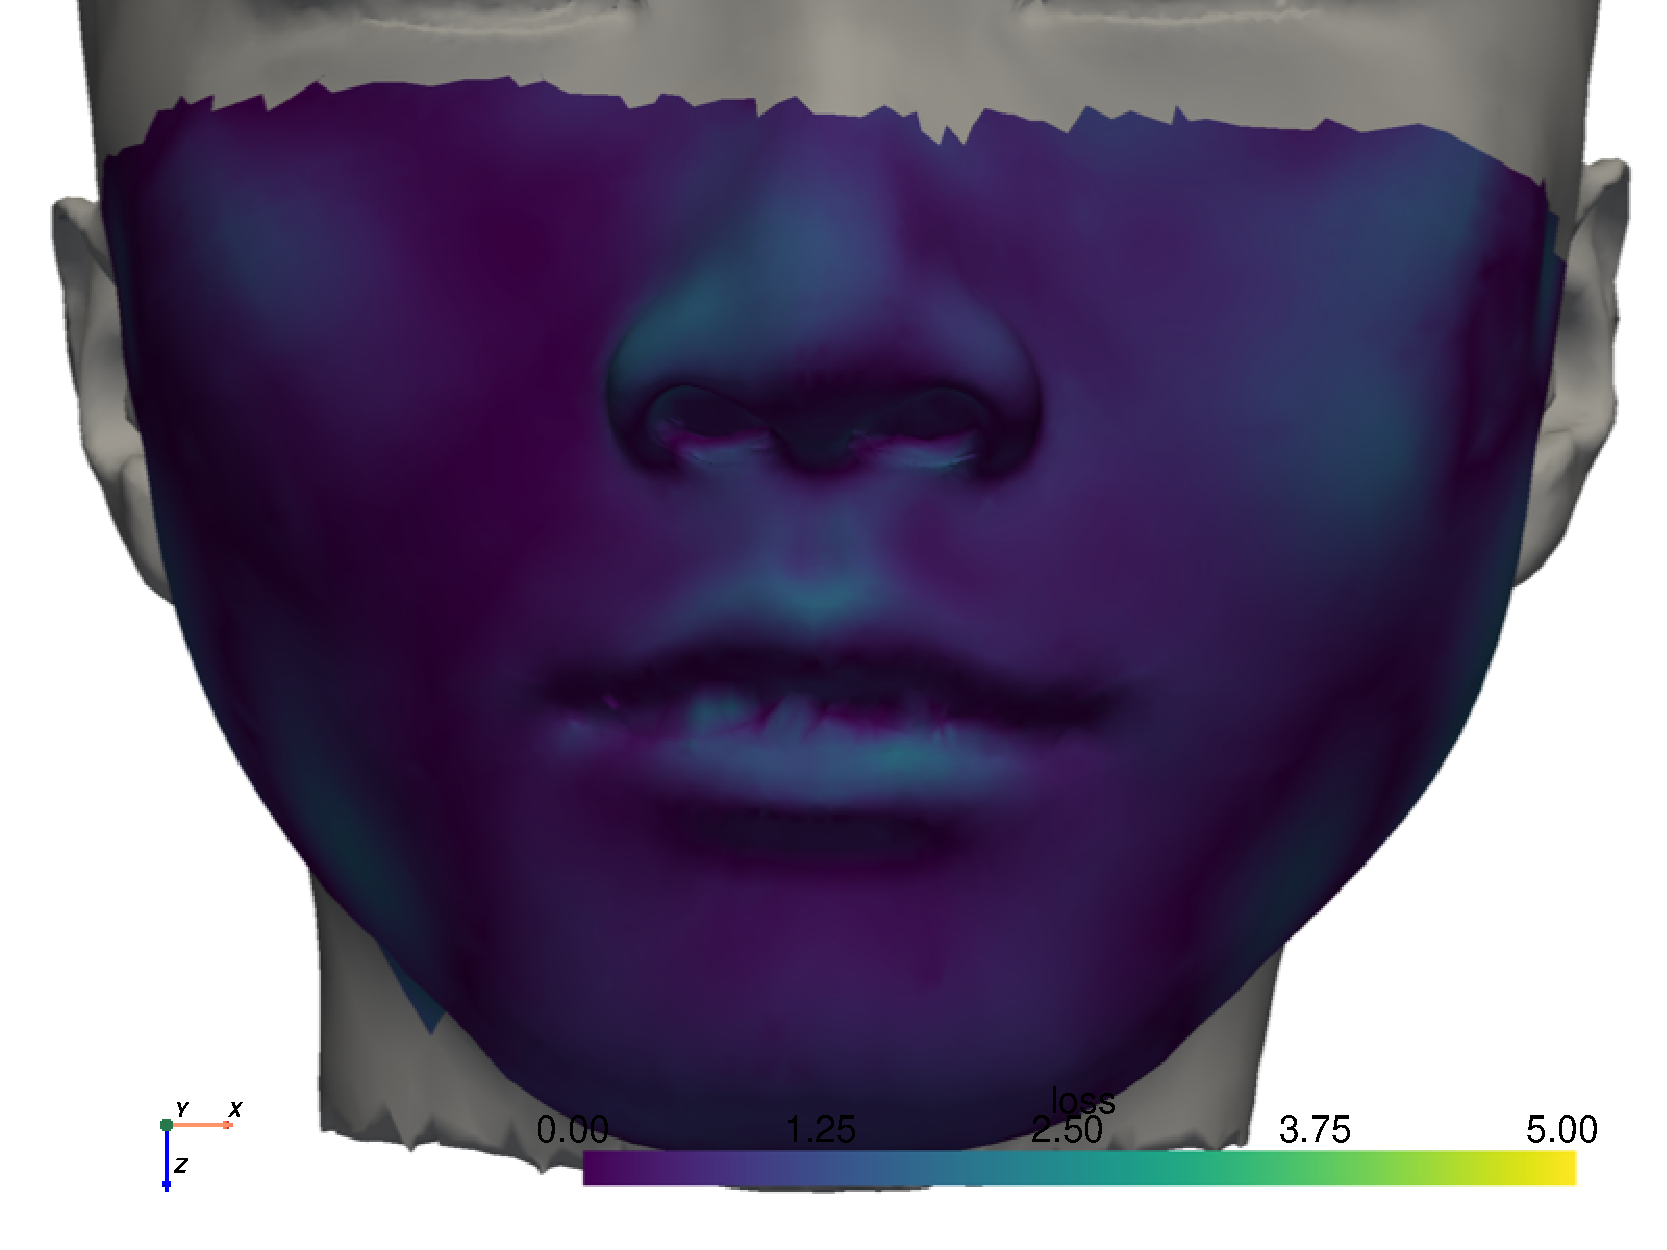
\includegraphics[height = 0.24 \linewidth]{fig/loss/112049.pdf}
    % 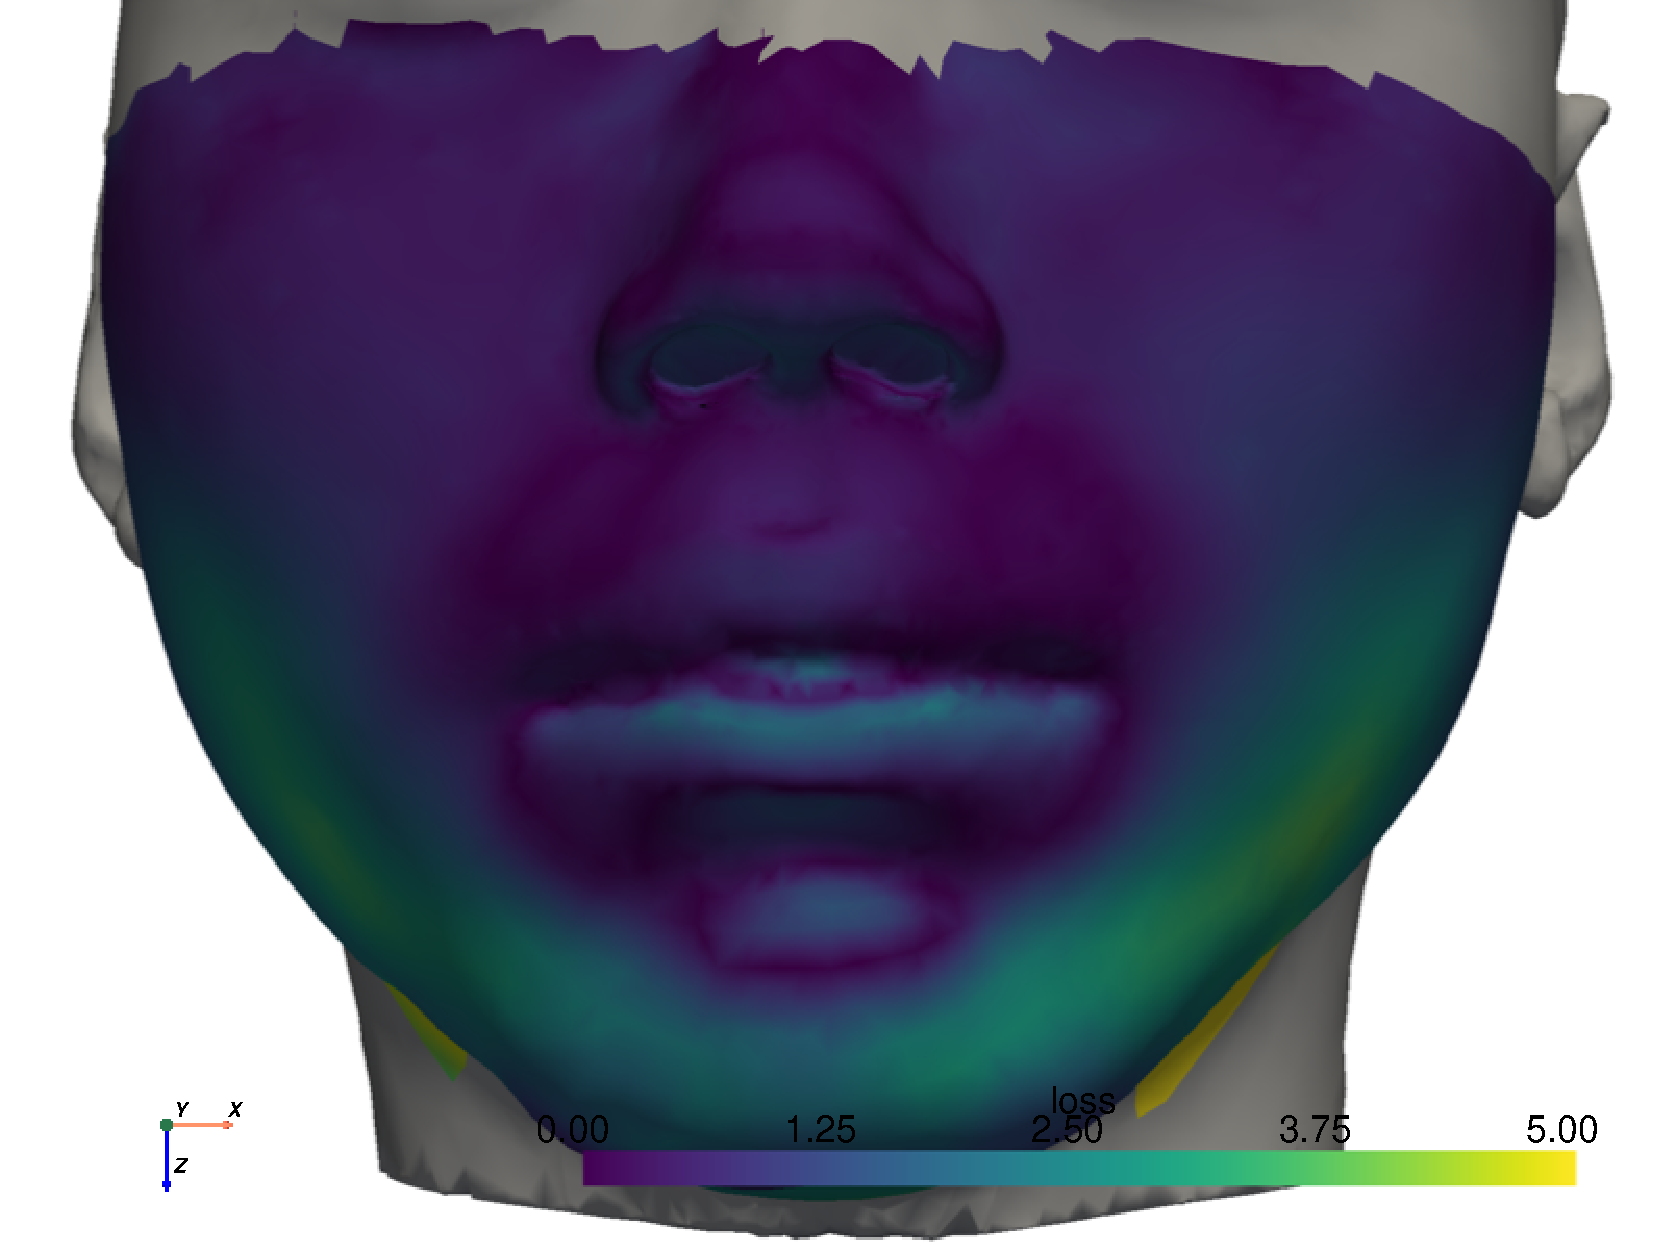
\includegraphics[height = 0.24 \linewidth]{fig/loss/112070.pdf}
    % 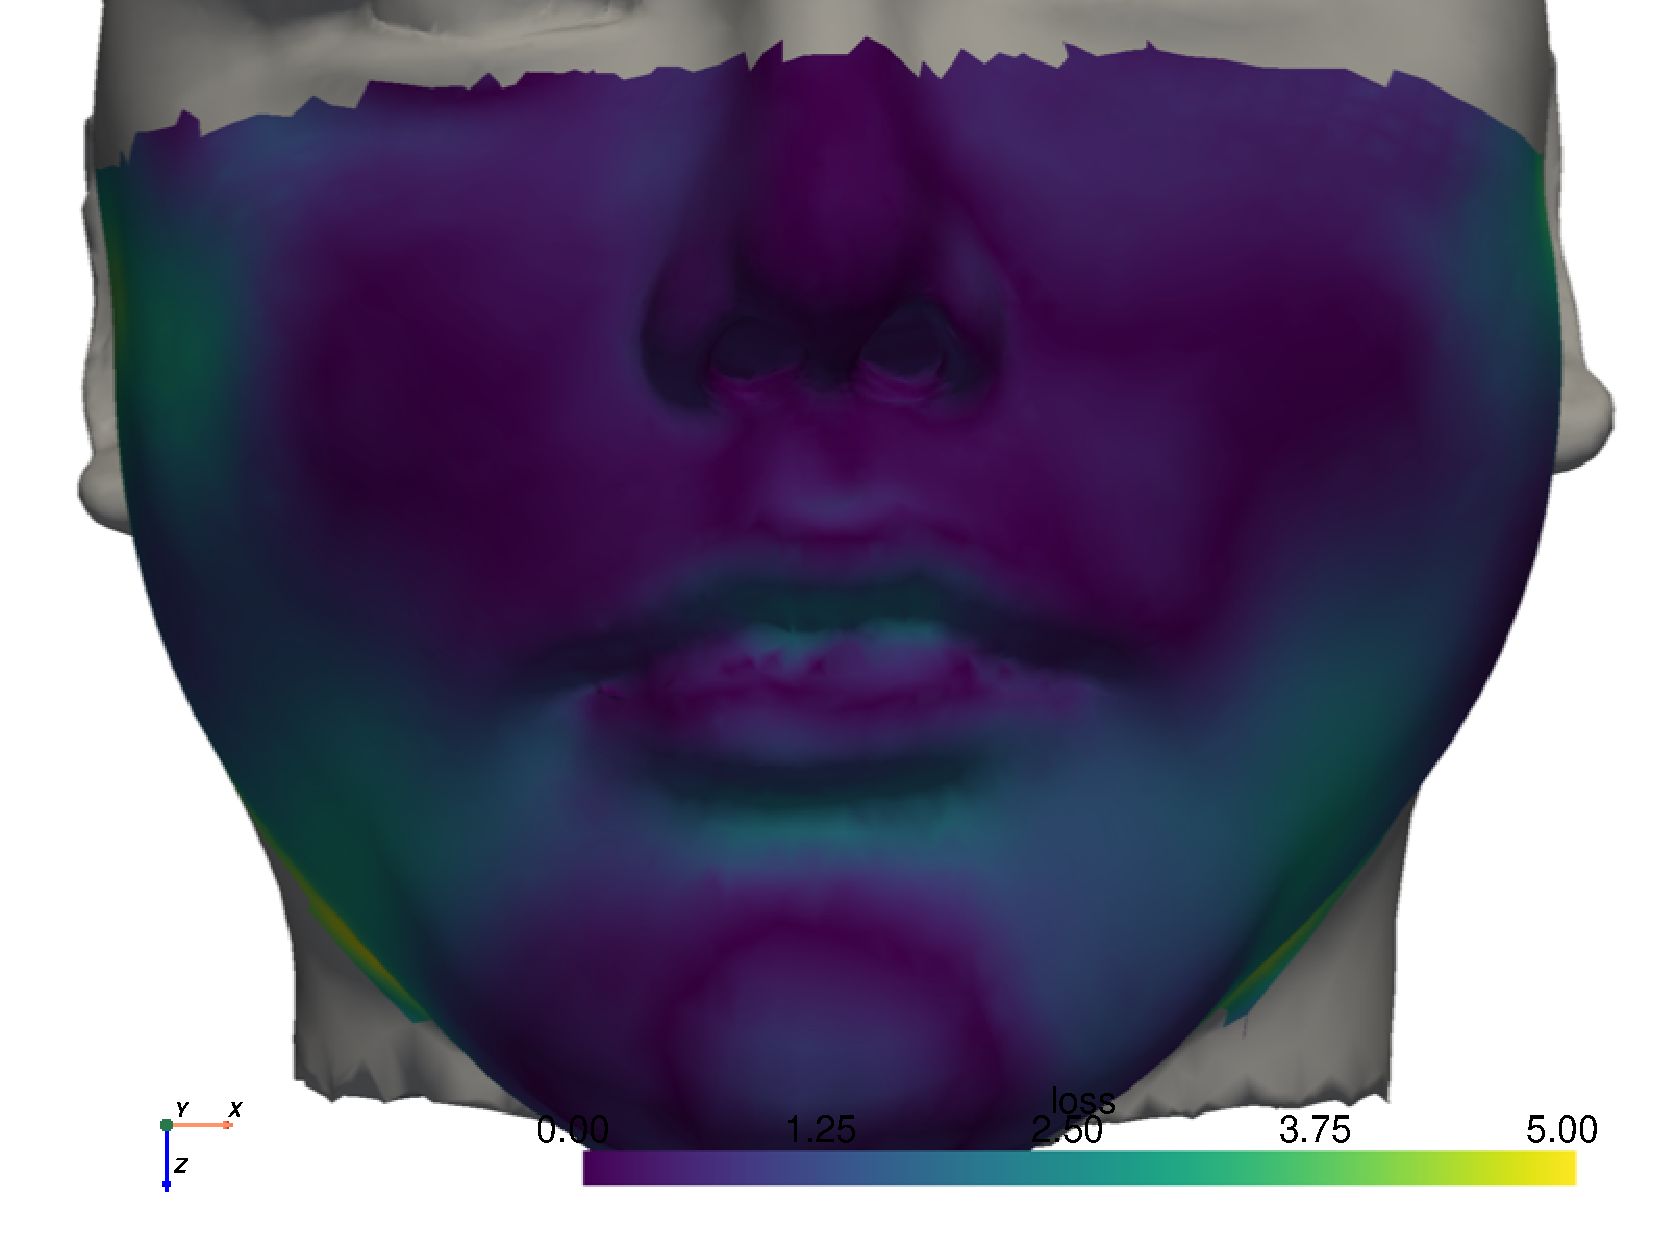
\includegraphics[height = 0.24 \linewidth]{fig/loss/113116.pdf}
    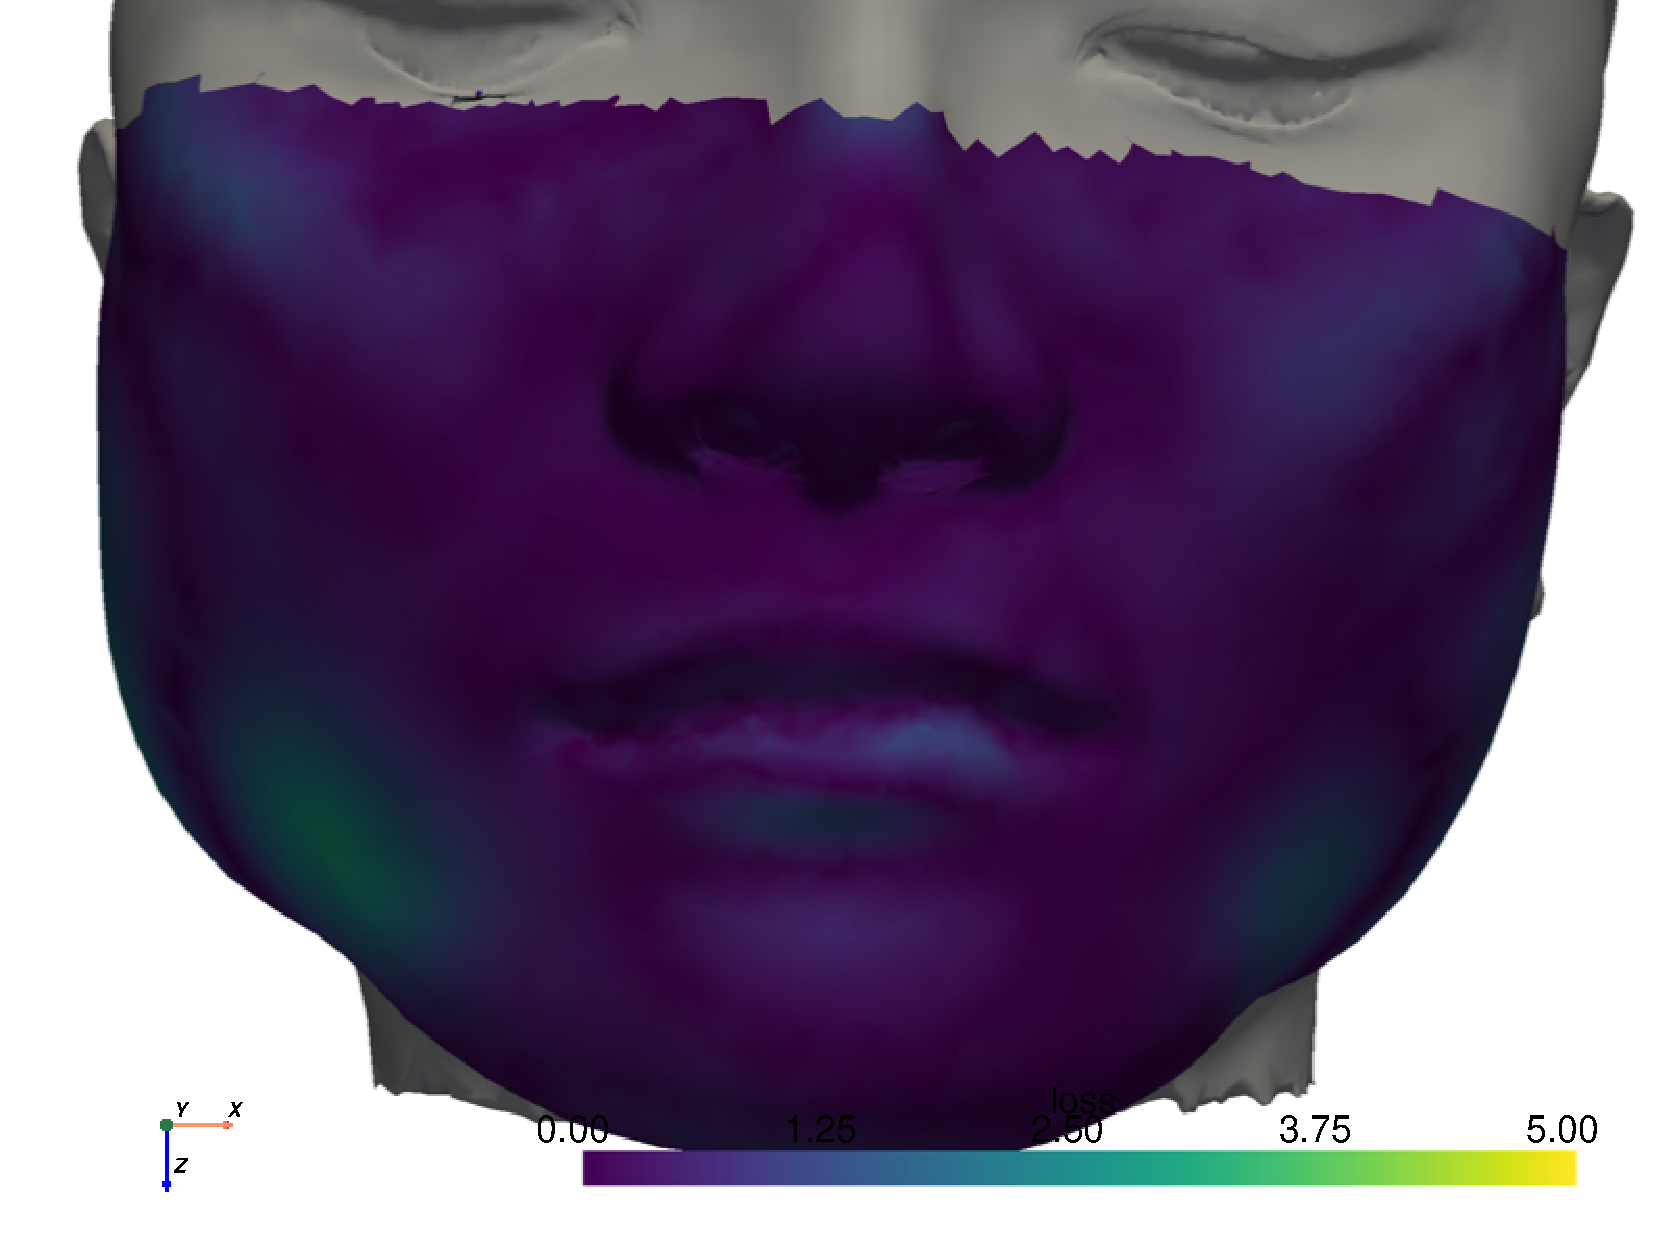
\includegraphics[height = 0.24 \linewidth]{fig/loss/113286.pdf}
    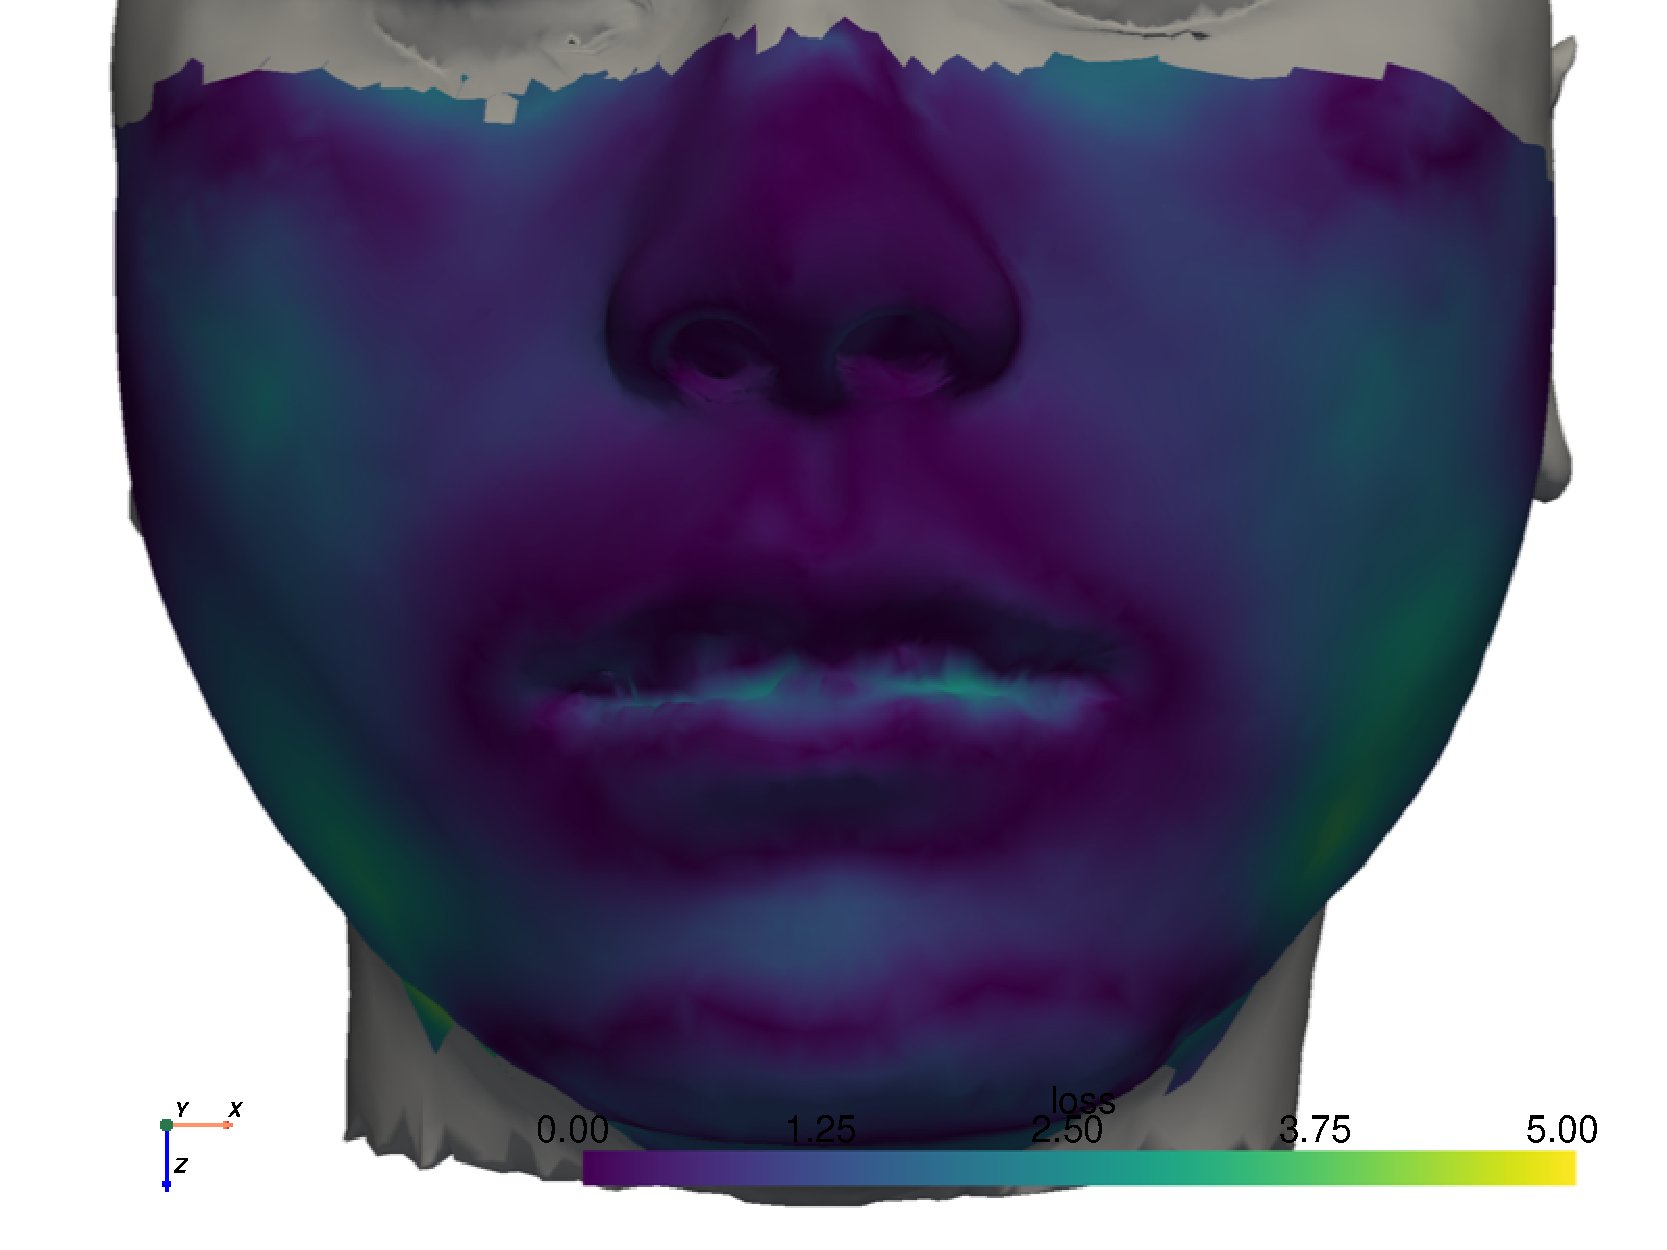
\includegraphics[height = 0.24 \linewidth]{fig/loss/113406.pdf}
    \\[2em]
    % 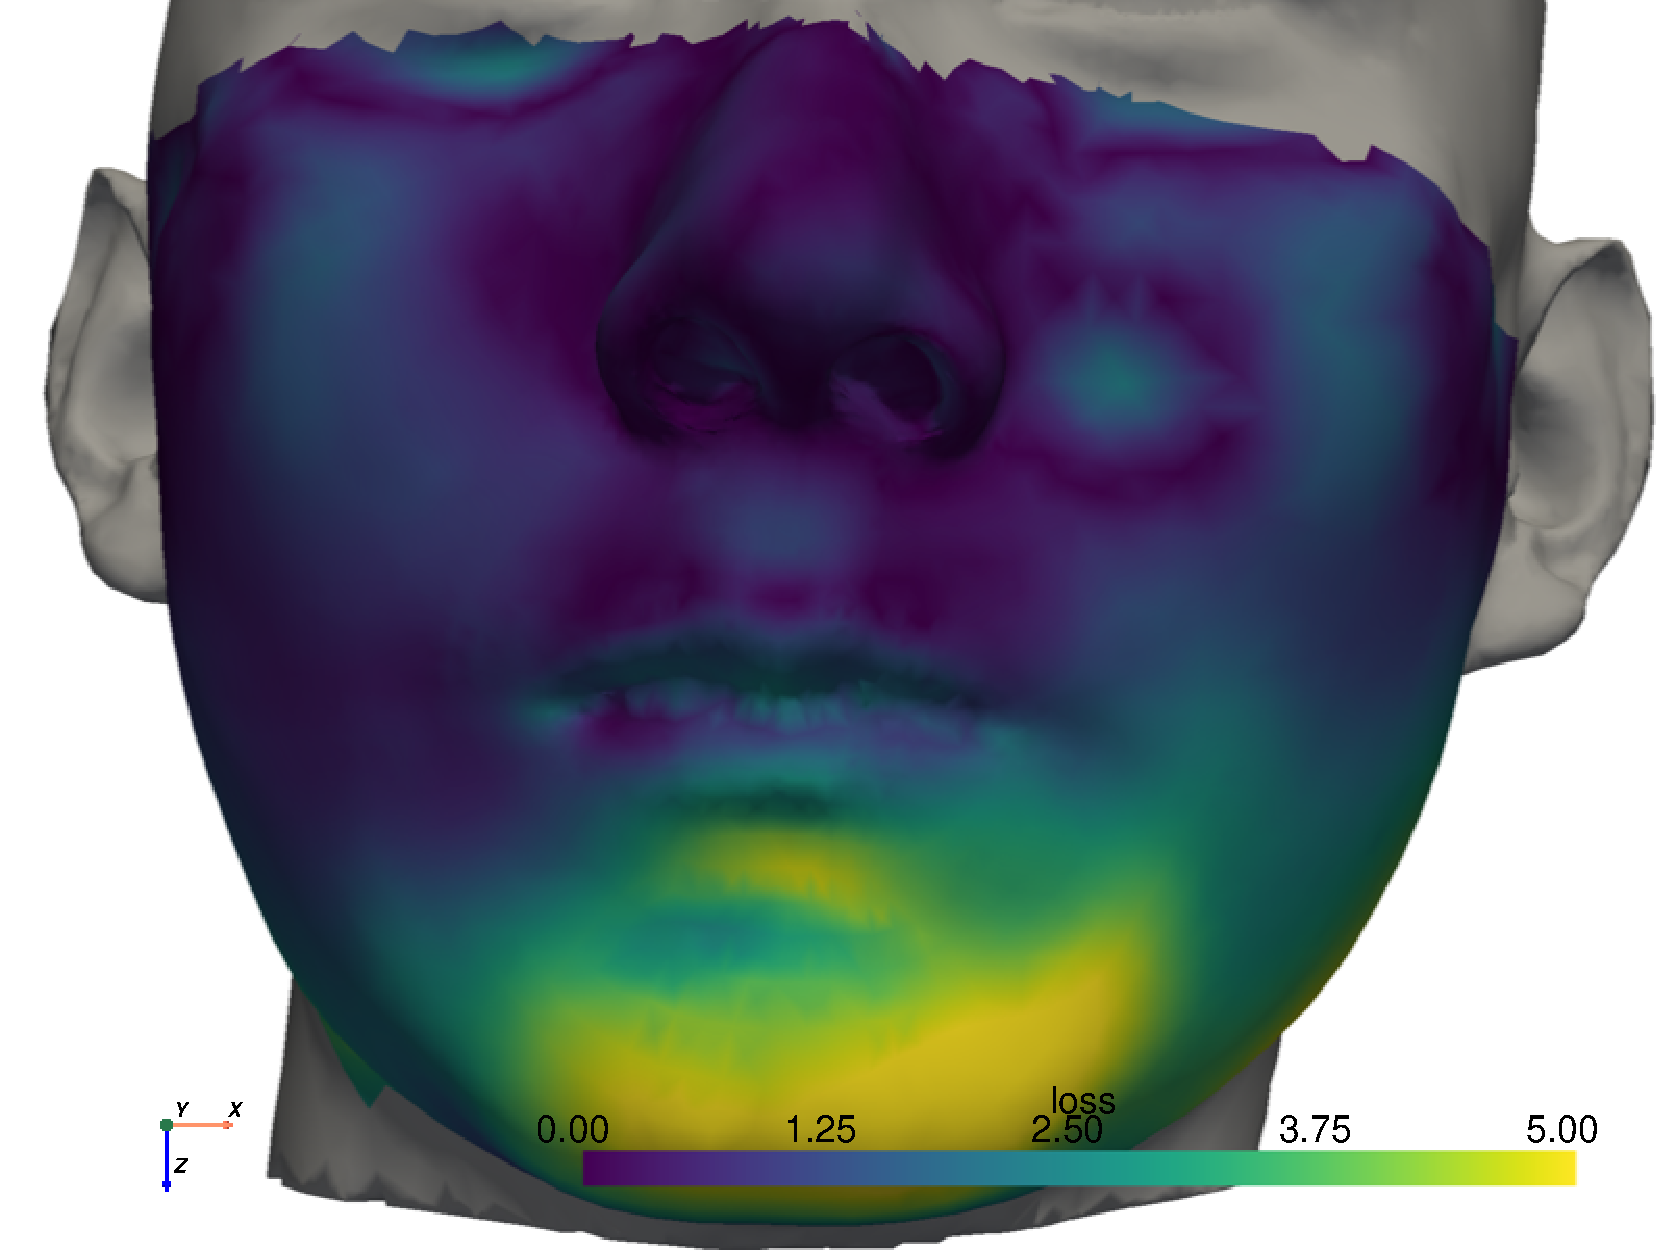
\includegraphics[height = 0.24 \linewidth]{fig/loss/118643.pdf}
    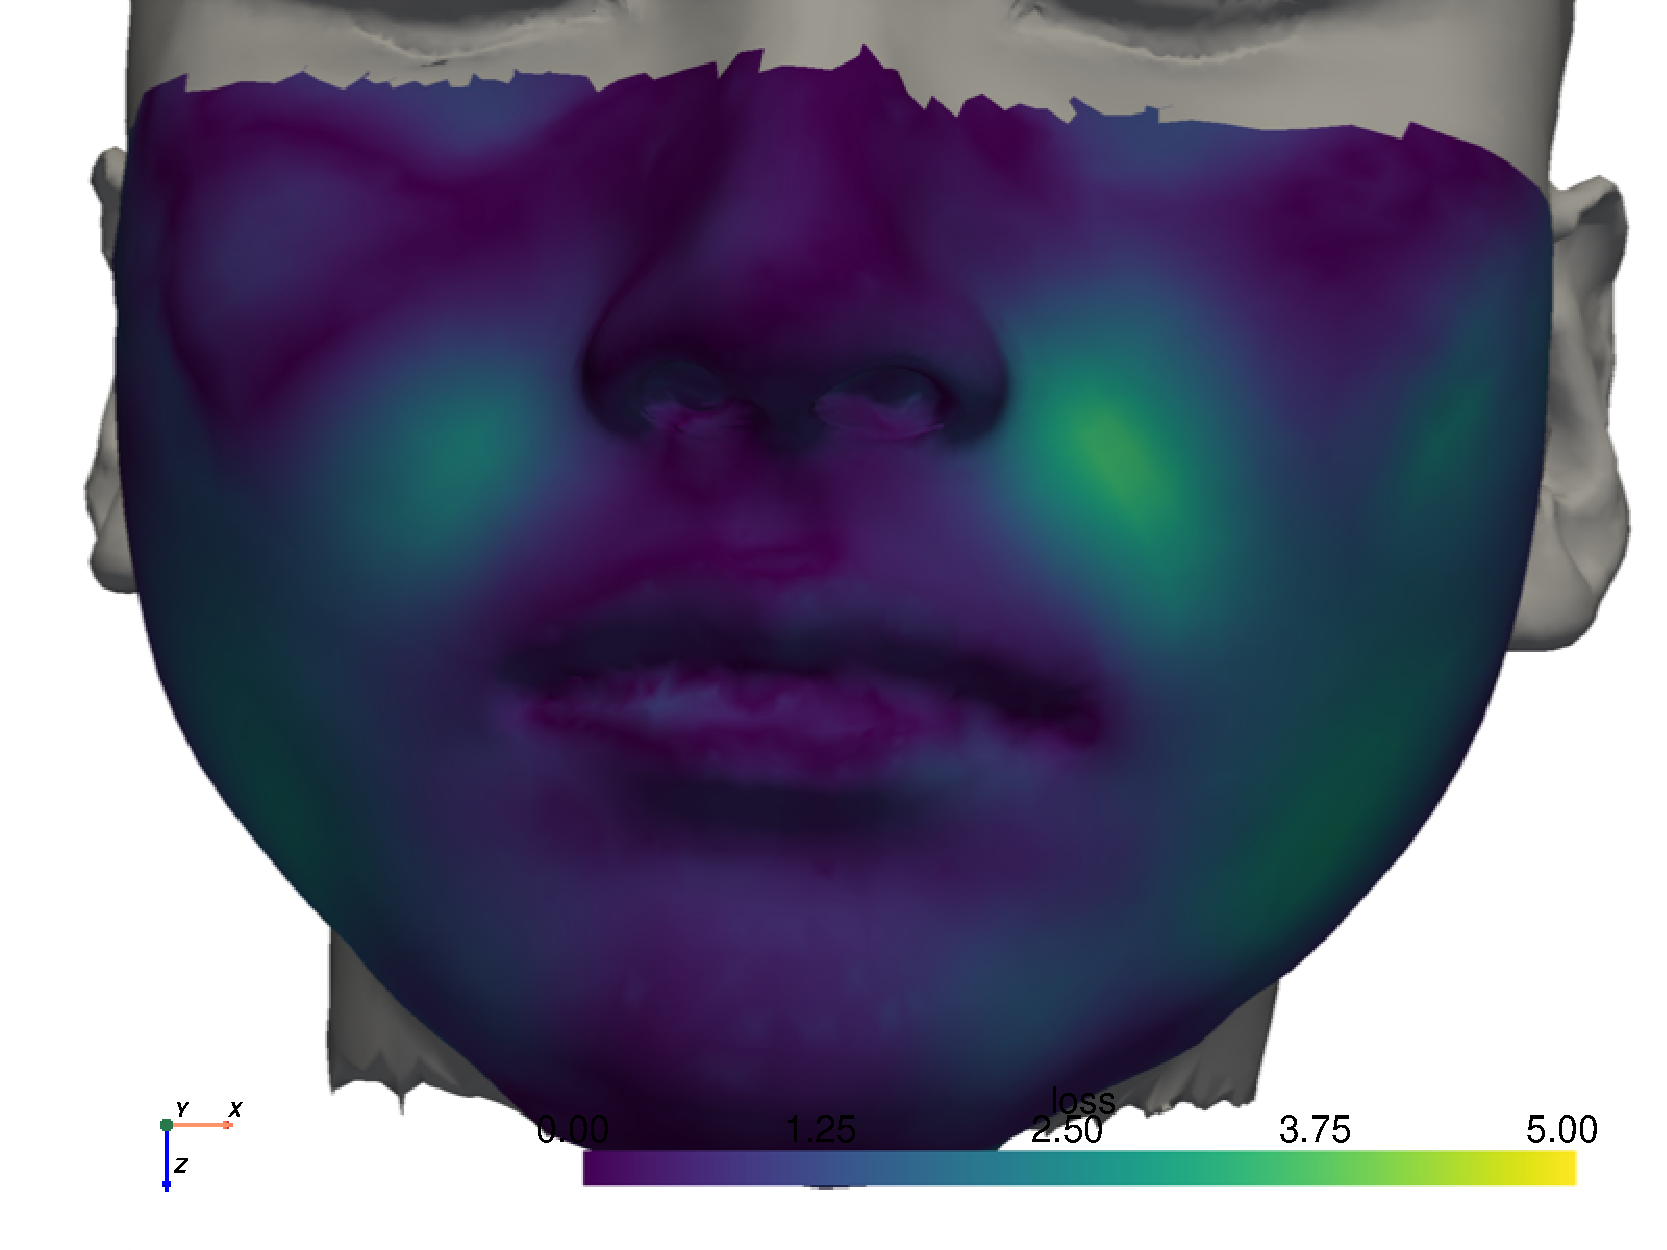
\includegraphics[height = 0.24 \linewidth]{fig/loss/118791.pdf}
    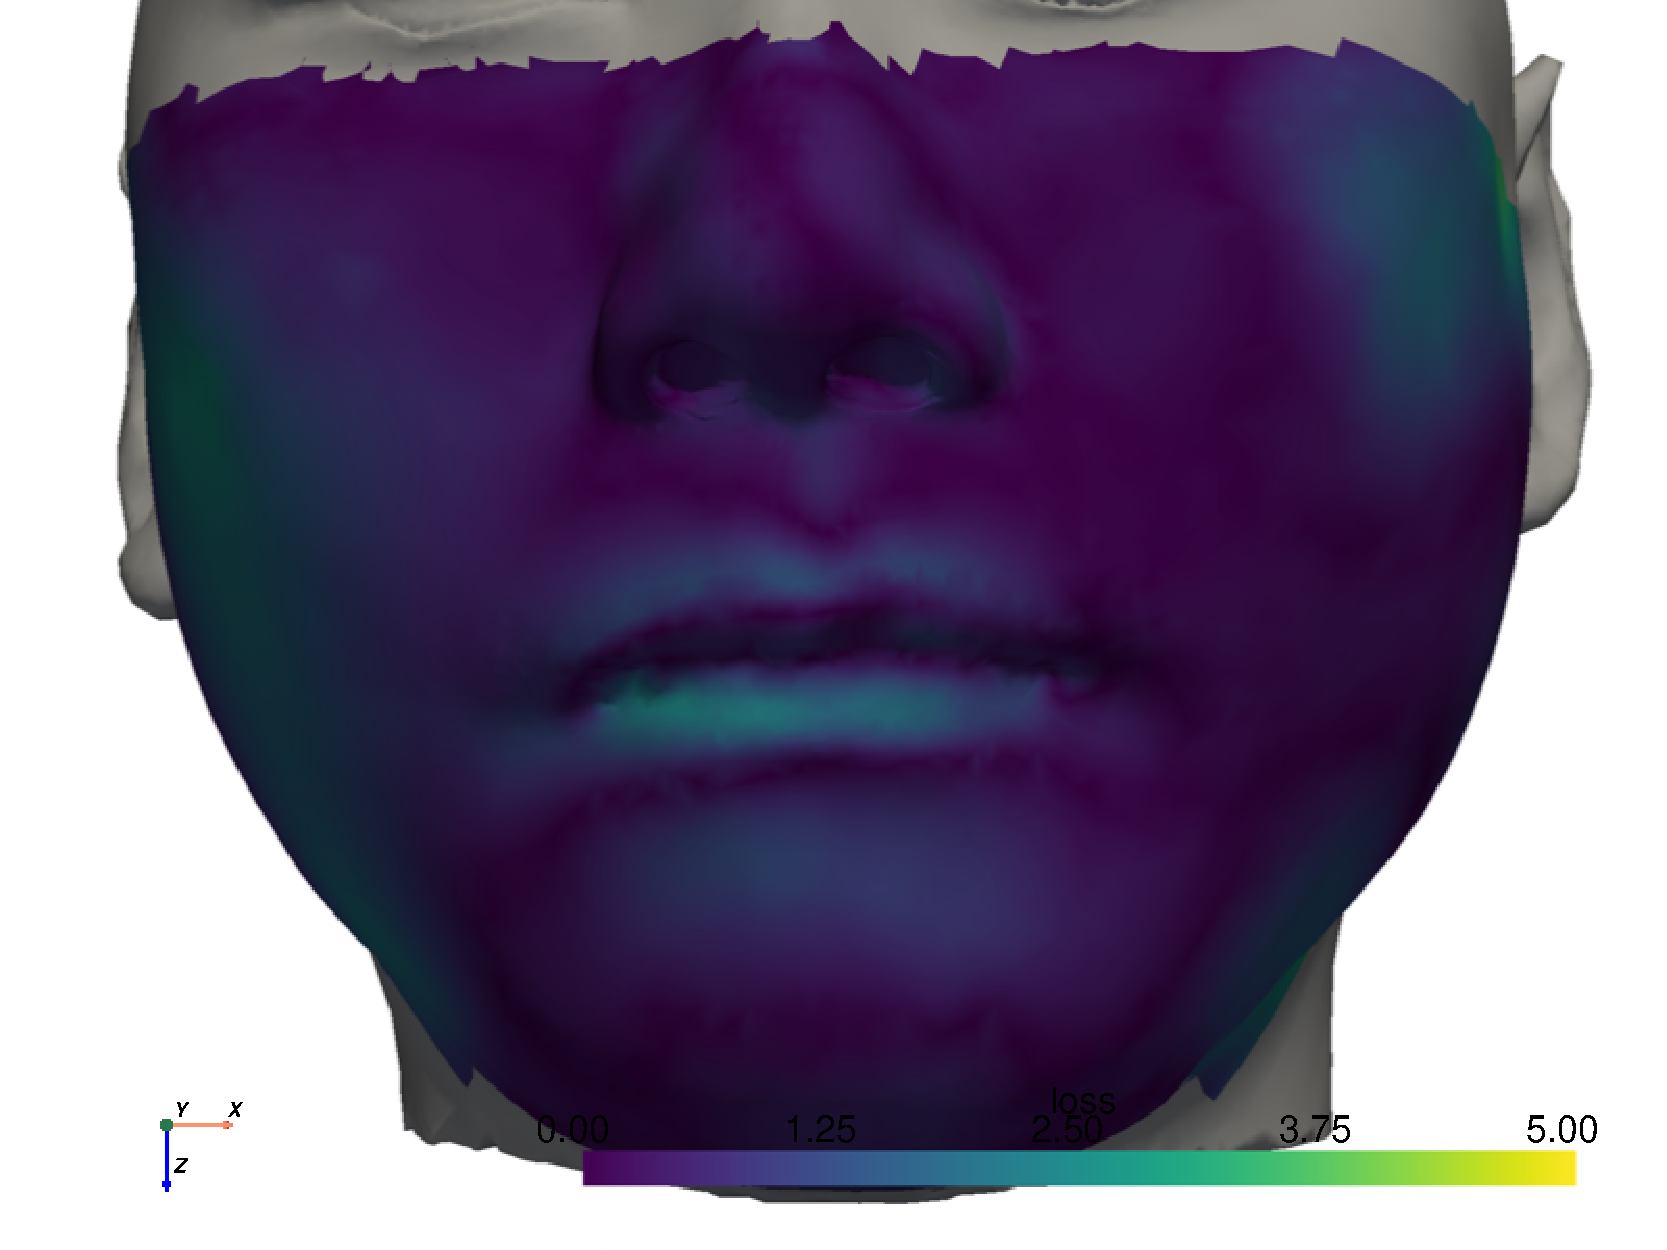
\includegraphics[height = 0.24 \linewidth]{fig/loss/119440.pdf}
    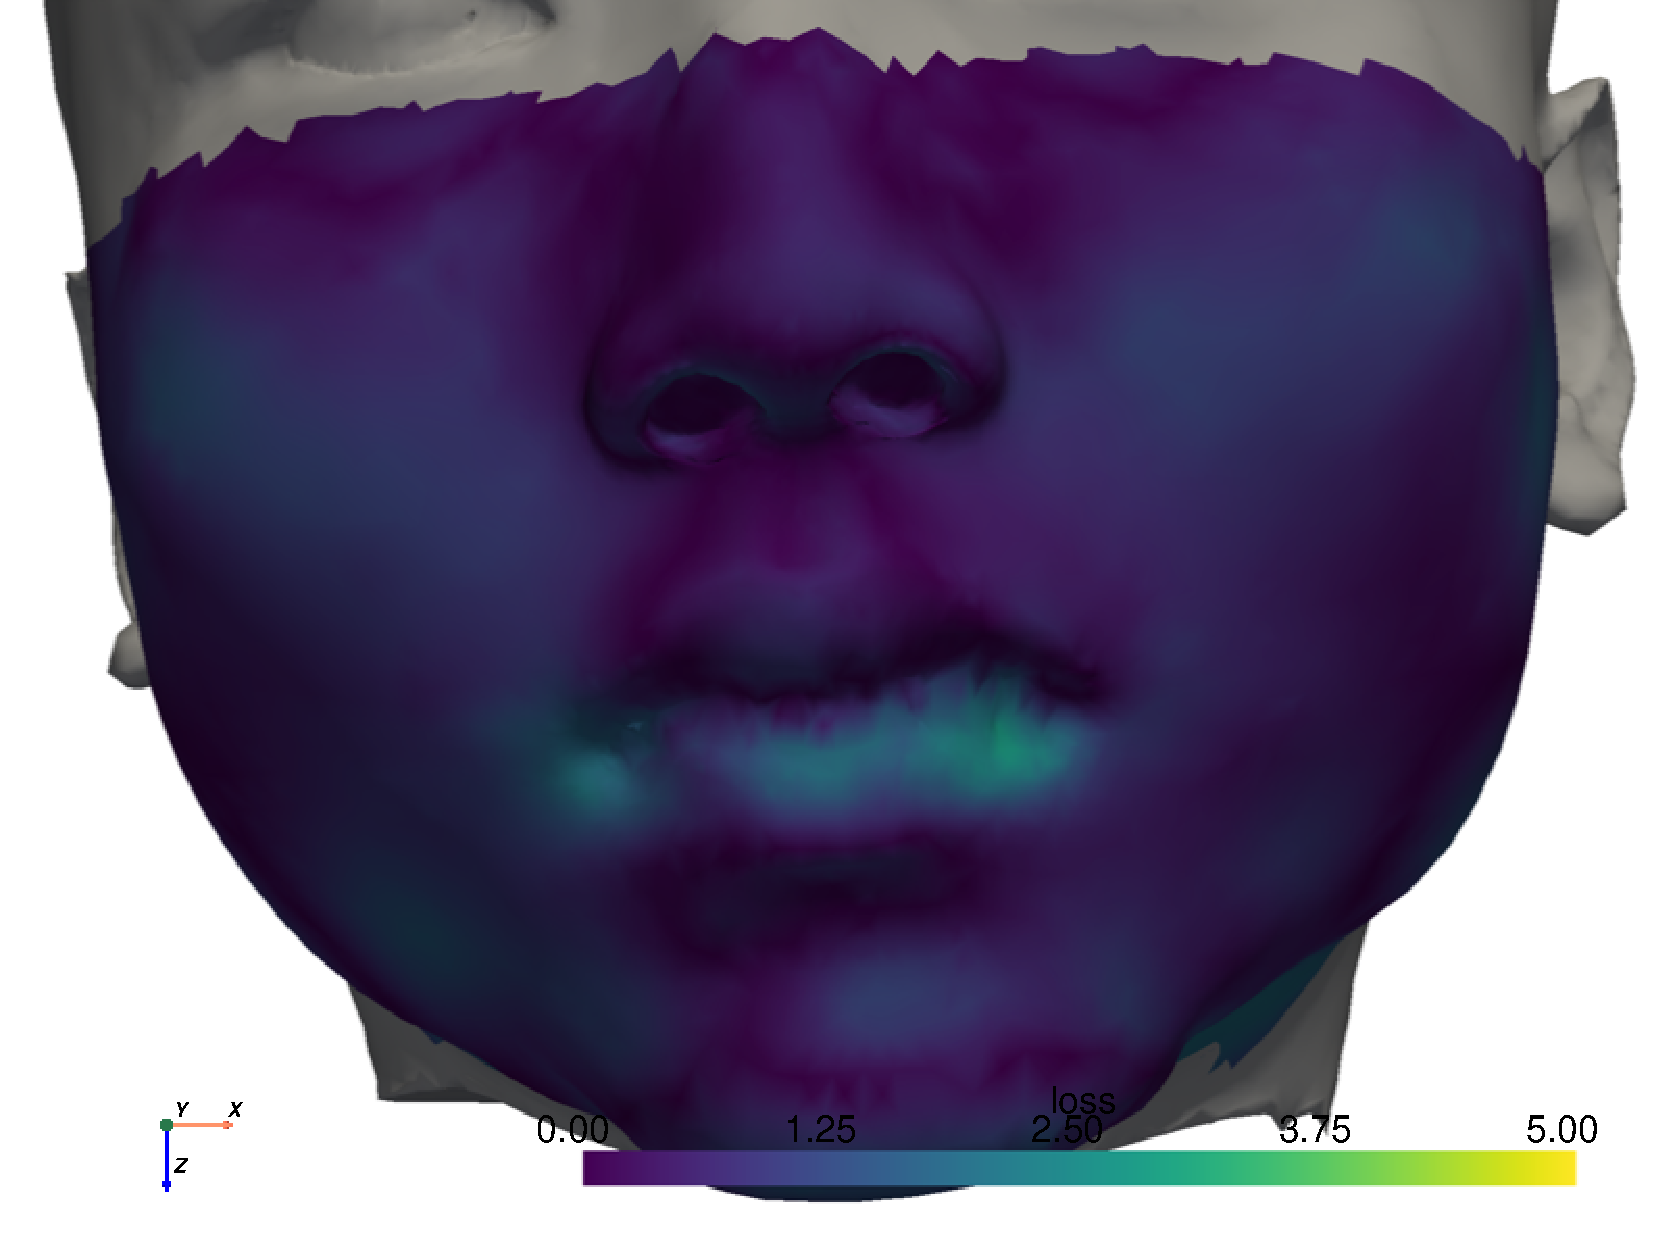
\includegraphics[height = 0.24 \linewidth]{fig/loss/120056.pdf}
  \end{figure}
\end{frame}

\section*{}

\begin{frame}
  \begin{center}
    \Huge\normalfont\bfseries
    恳请各位老师批评指正! \\
  \end{center}
  % \begin{tcolorbox}[
  %     colback = tsinghua,
  %     coltext = white,
  %     boxrule = 0pt,
  %   ]
  \begin{center}
    \normalfont
    \Large 基于物理模拟的正颌手术术后外形预测 \\
    \normalsize 毕业设计终期汇报
  \end{center}
  % \end{tcolorbox}
\end{frame}

\end{document}
